% !TEX root = presentation.tex
	\begin{frame}\frametitle{Overview}
		\begin{columns}
			\begin{column}{0.9\textwidth}
				\begin{center}
					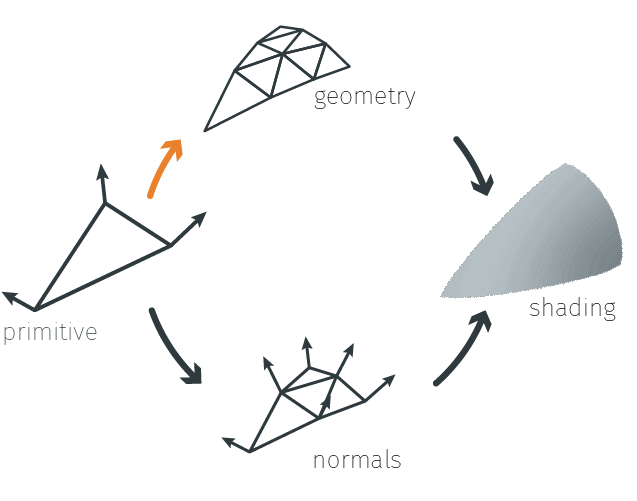
\includegraphics[width=\textwidth]{./img/1_single/recap_inputToGeom.png}
				\end{center}		
			\end{column}
		\end{columns}
	\end{frame}	

	\begin{frame}\frametitle{Geometry}
		\enhancement{emphasize vertices better}
		\begin{columns}
			\begin{column}{0.6\textwidth}
				\begin{center}
					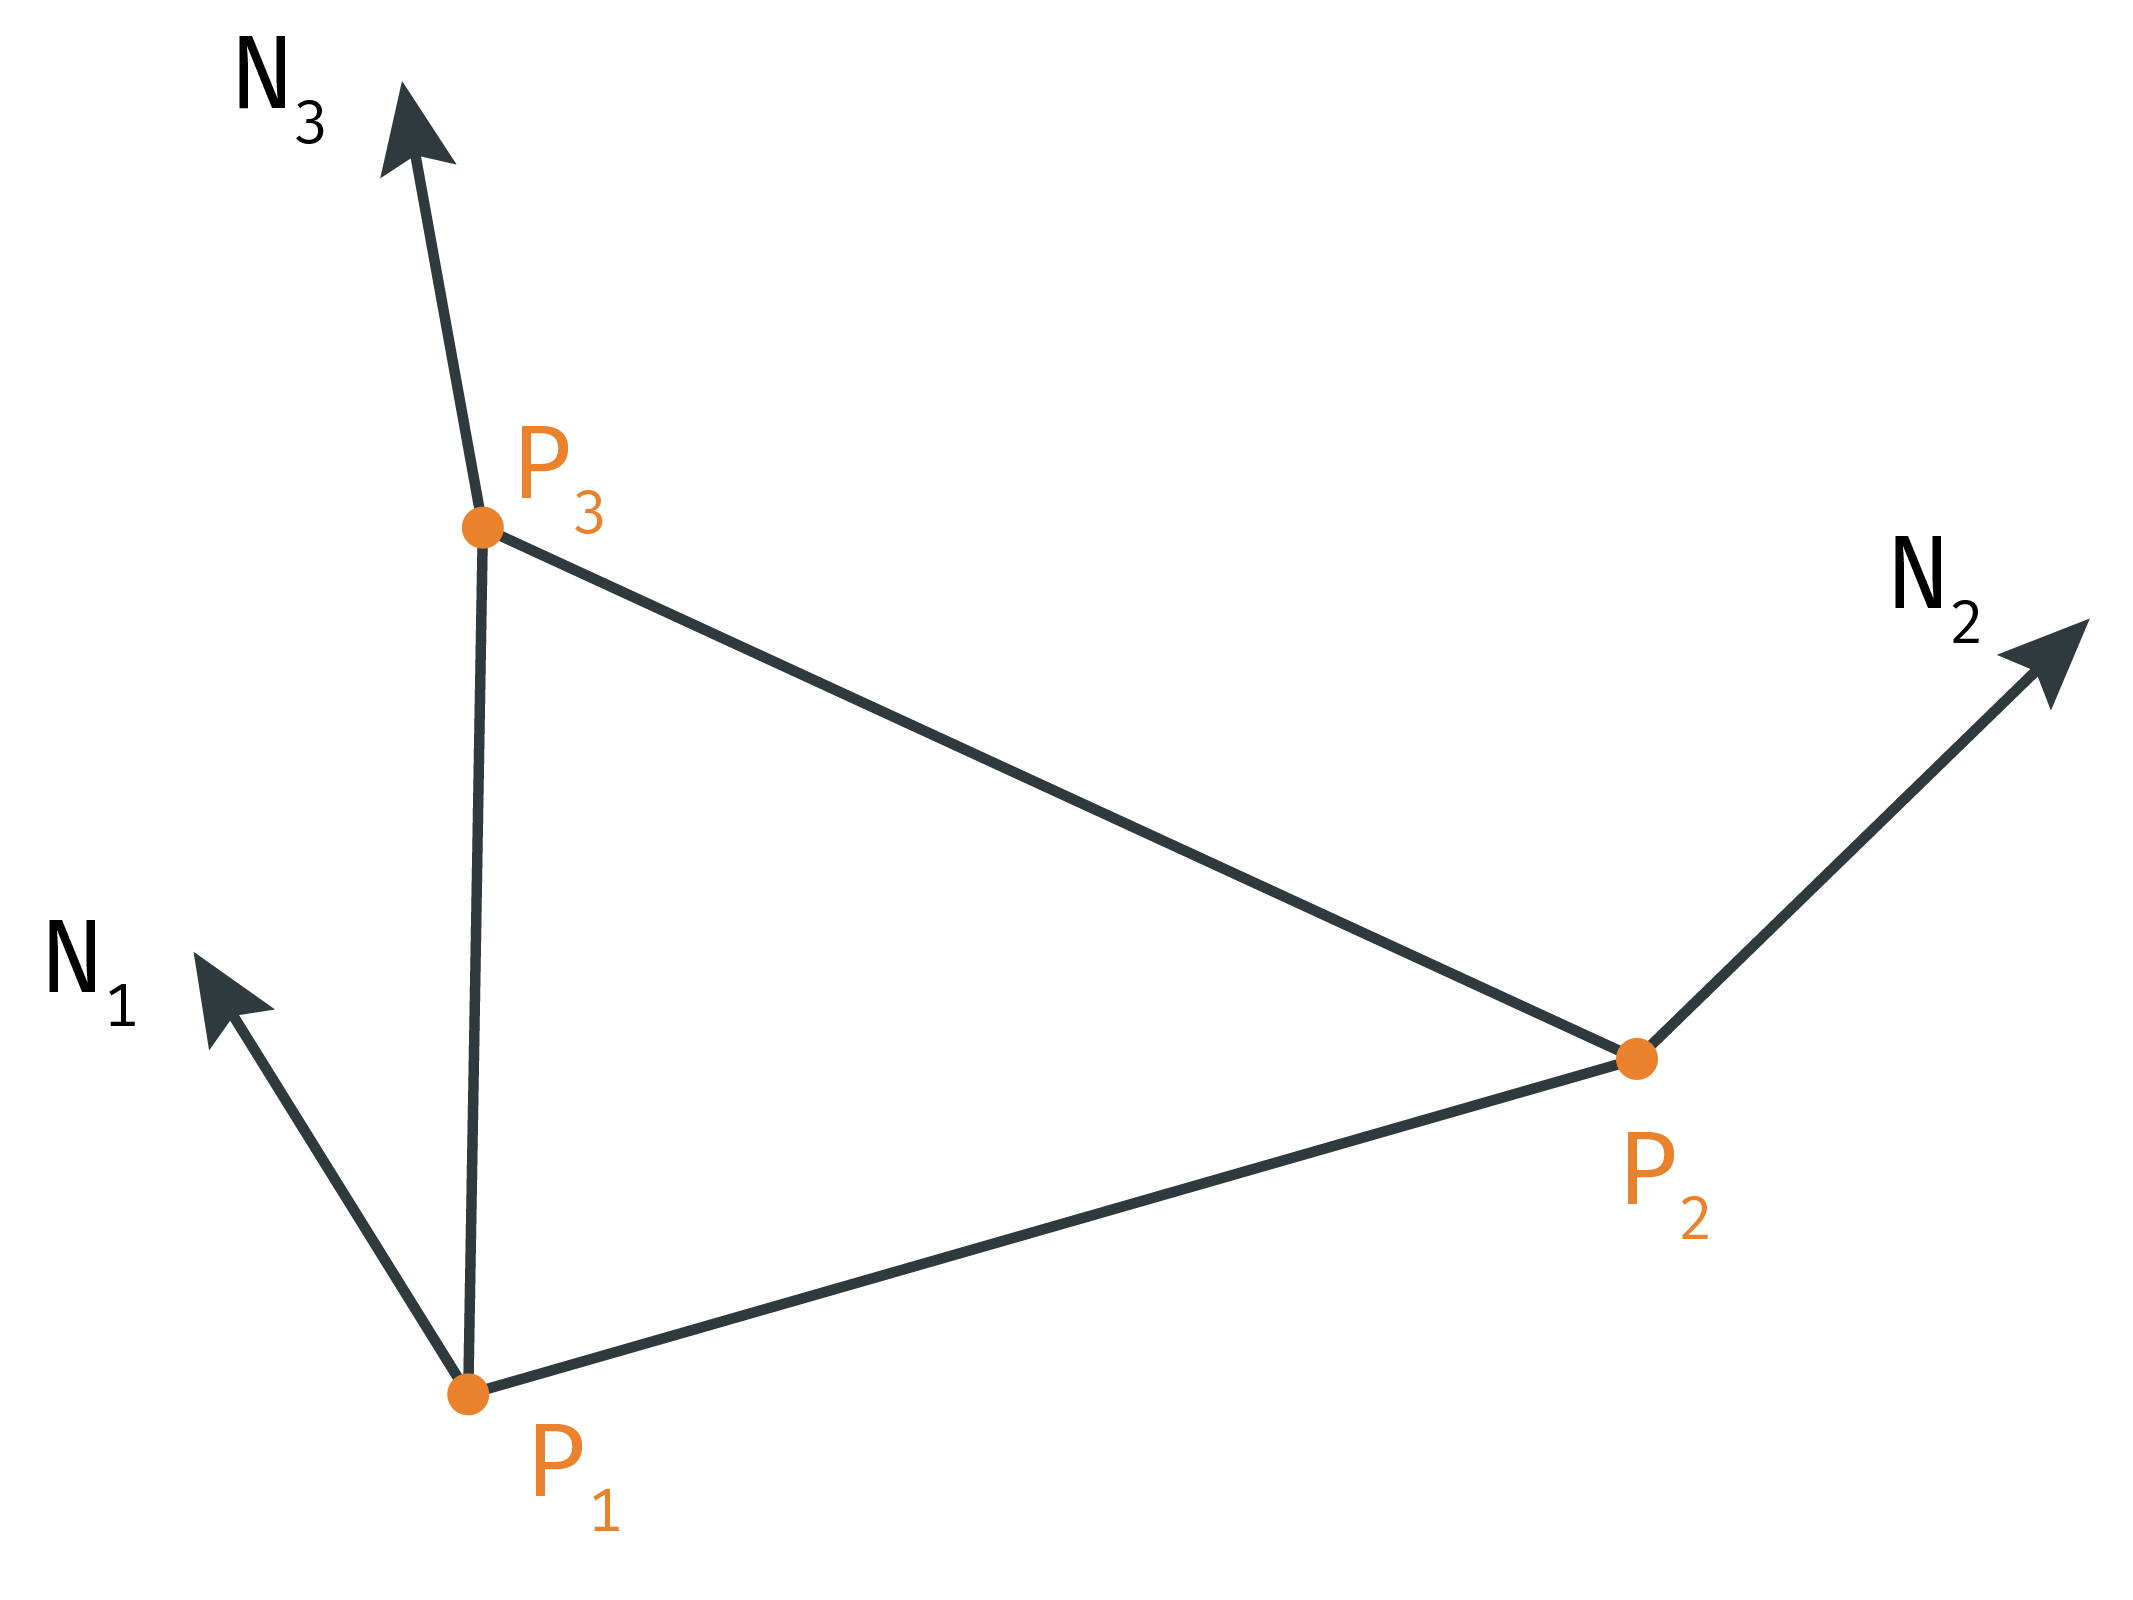
\includegraphics[width=\textwidth]{img/1_single/inputPrimitive_emphGeometry.png}
					\small{input primitive}
				\end{center}
			\end{column}
		\end{columns}
	\end{frame}

	% Geometry process
	\begin{frame}\frametitle{Geometry - Vertex Coefficients}
		\begin{columns}
			\begin{column}{0.6\textwidth}
				\begin{center}
					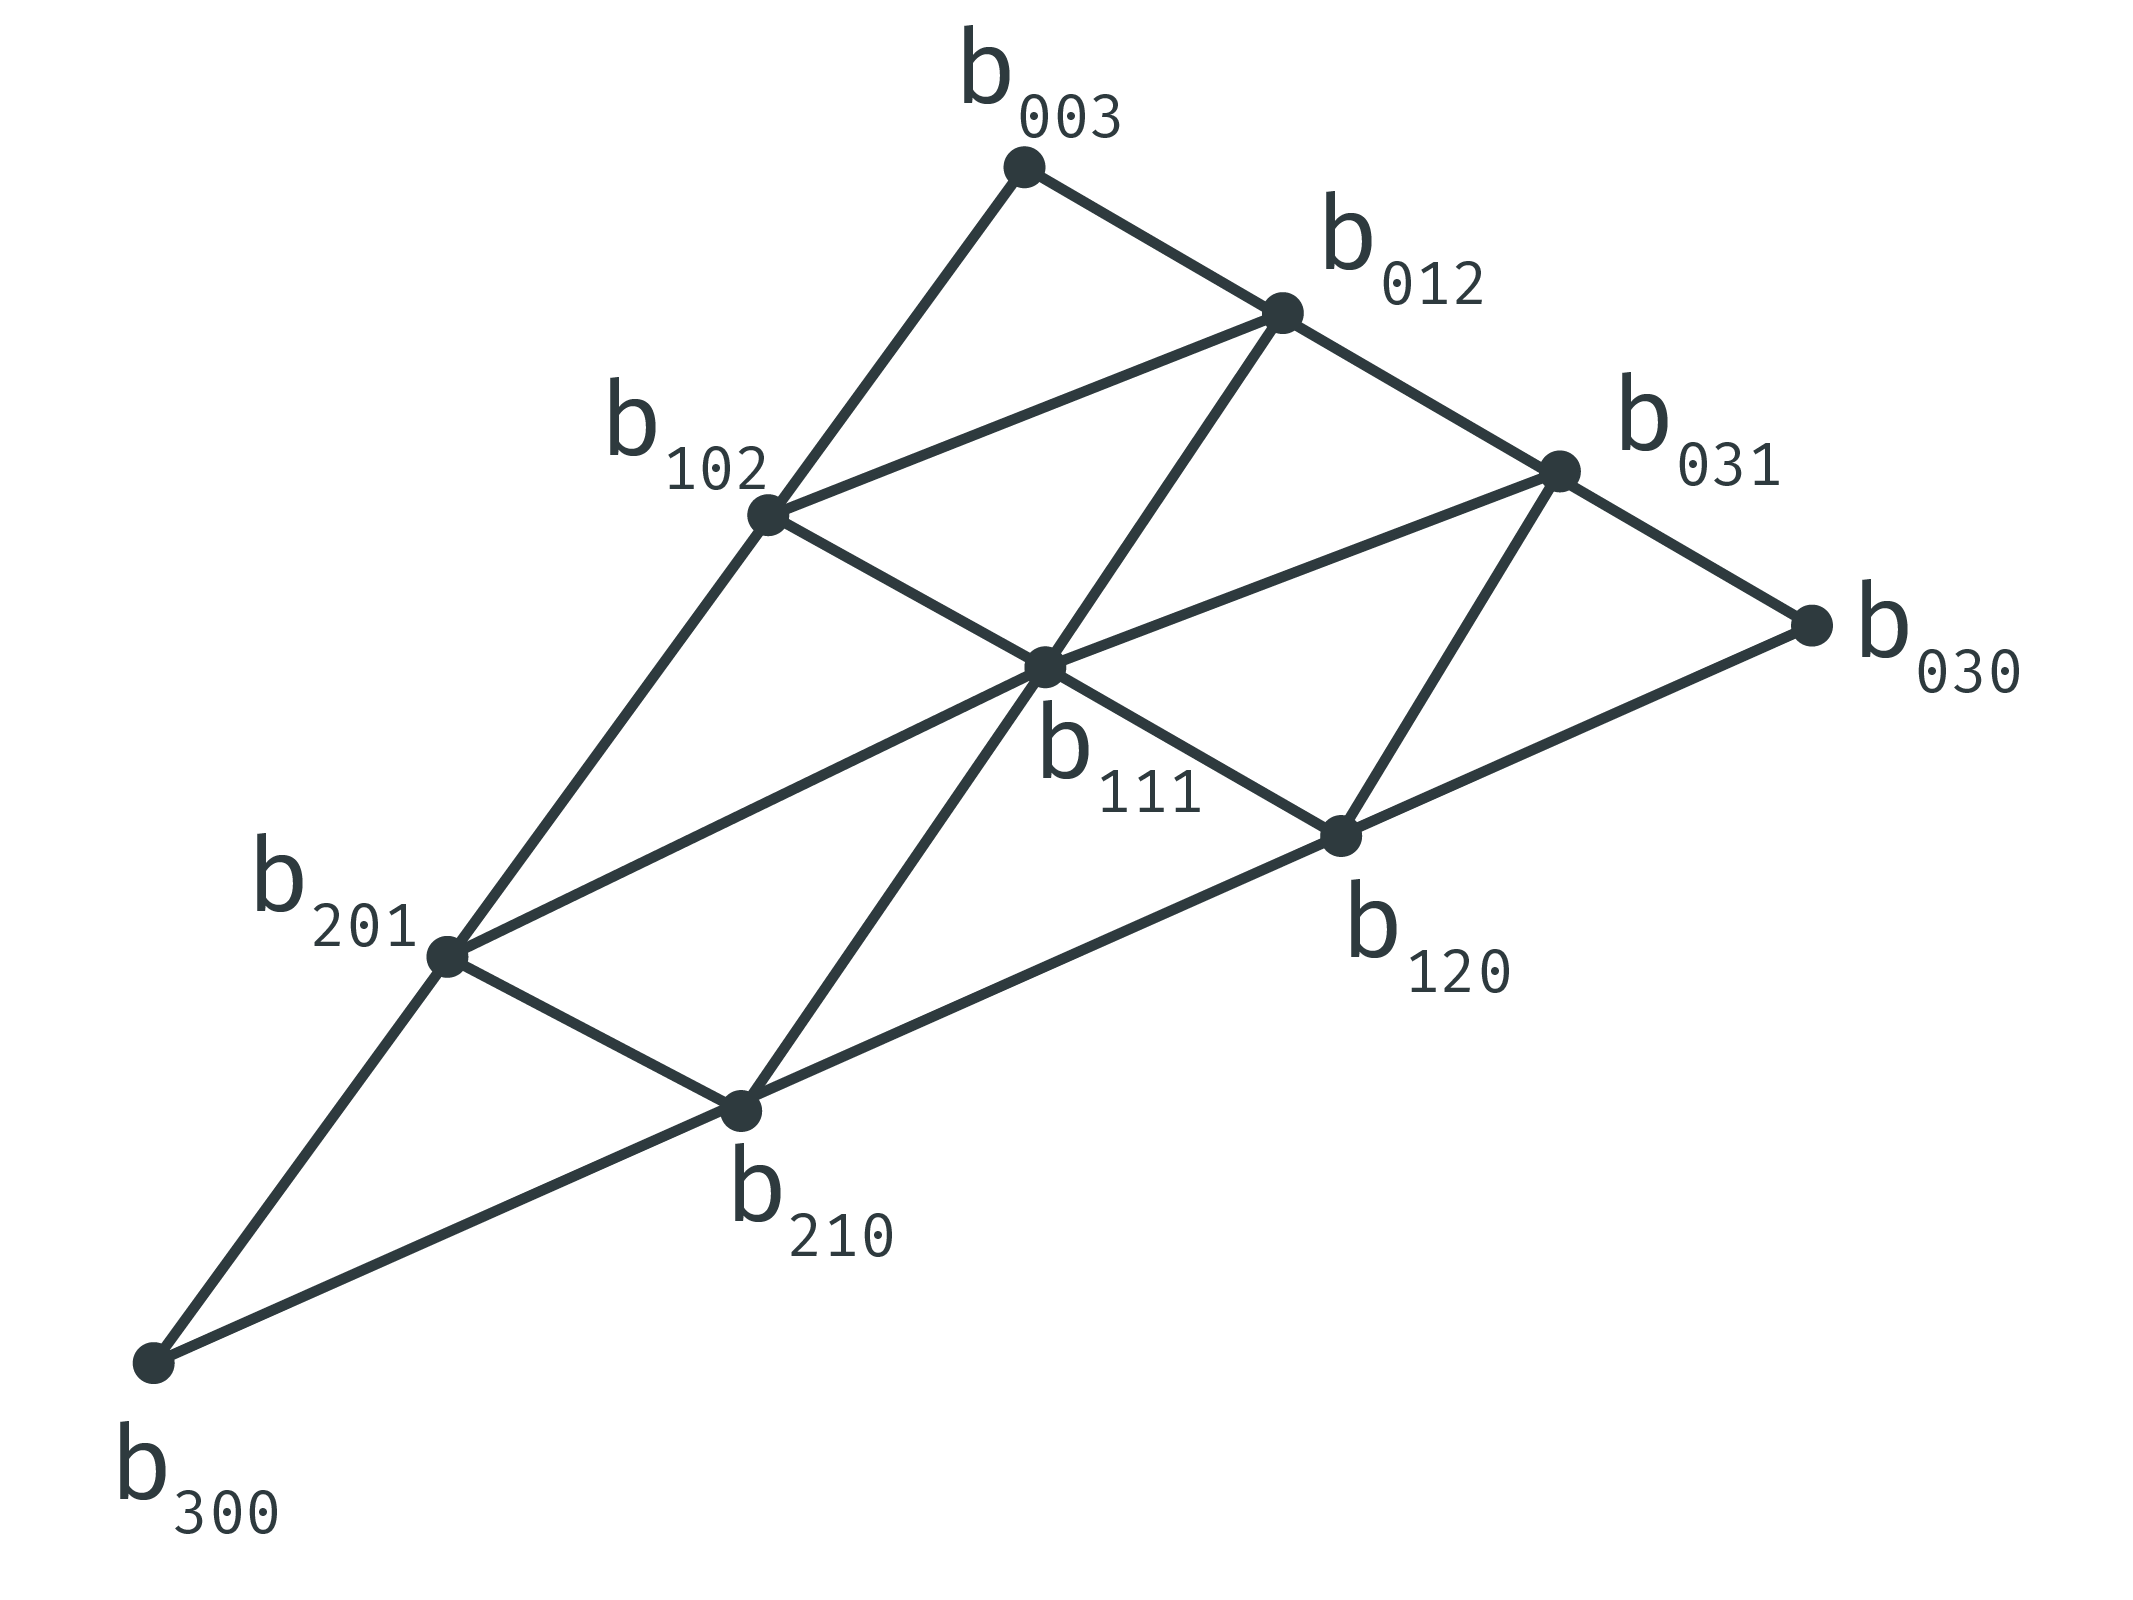
\includegraphics[width=\textwidth]{img/1_single/geometry_1.png}
					\small{control net}
				\end{center}
			\end{column}
				\begin{column}{0.4\textwidth}
					\uncover<2,3>{
					\begin{equation*}
						b_{ijk} = (iP_1 + jP_2 + kP_3)/3
					\end{equation*}
					}
					\uncover<3>{
					\begin{equation*}
						\begin{aligned}
						b_{300} & = P_1,\\
						b_{030} & = P_2,\\
						b_{003} & = P_3
						\end{aligned}
					\end{equation*}
					}
				\end{column}
		\end{columns}
	\end{frame}

	\begin{frame}\frametitle{Geometry - Tangent Coefficients}
		\begin{columns}
			\begin{column}{0.6\textwidth}
				\begin{center}
				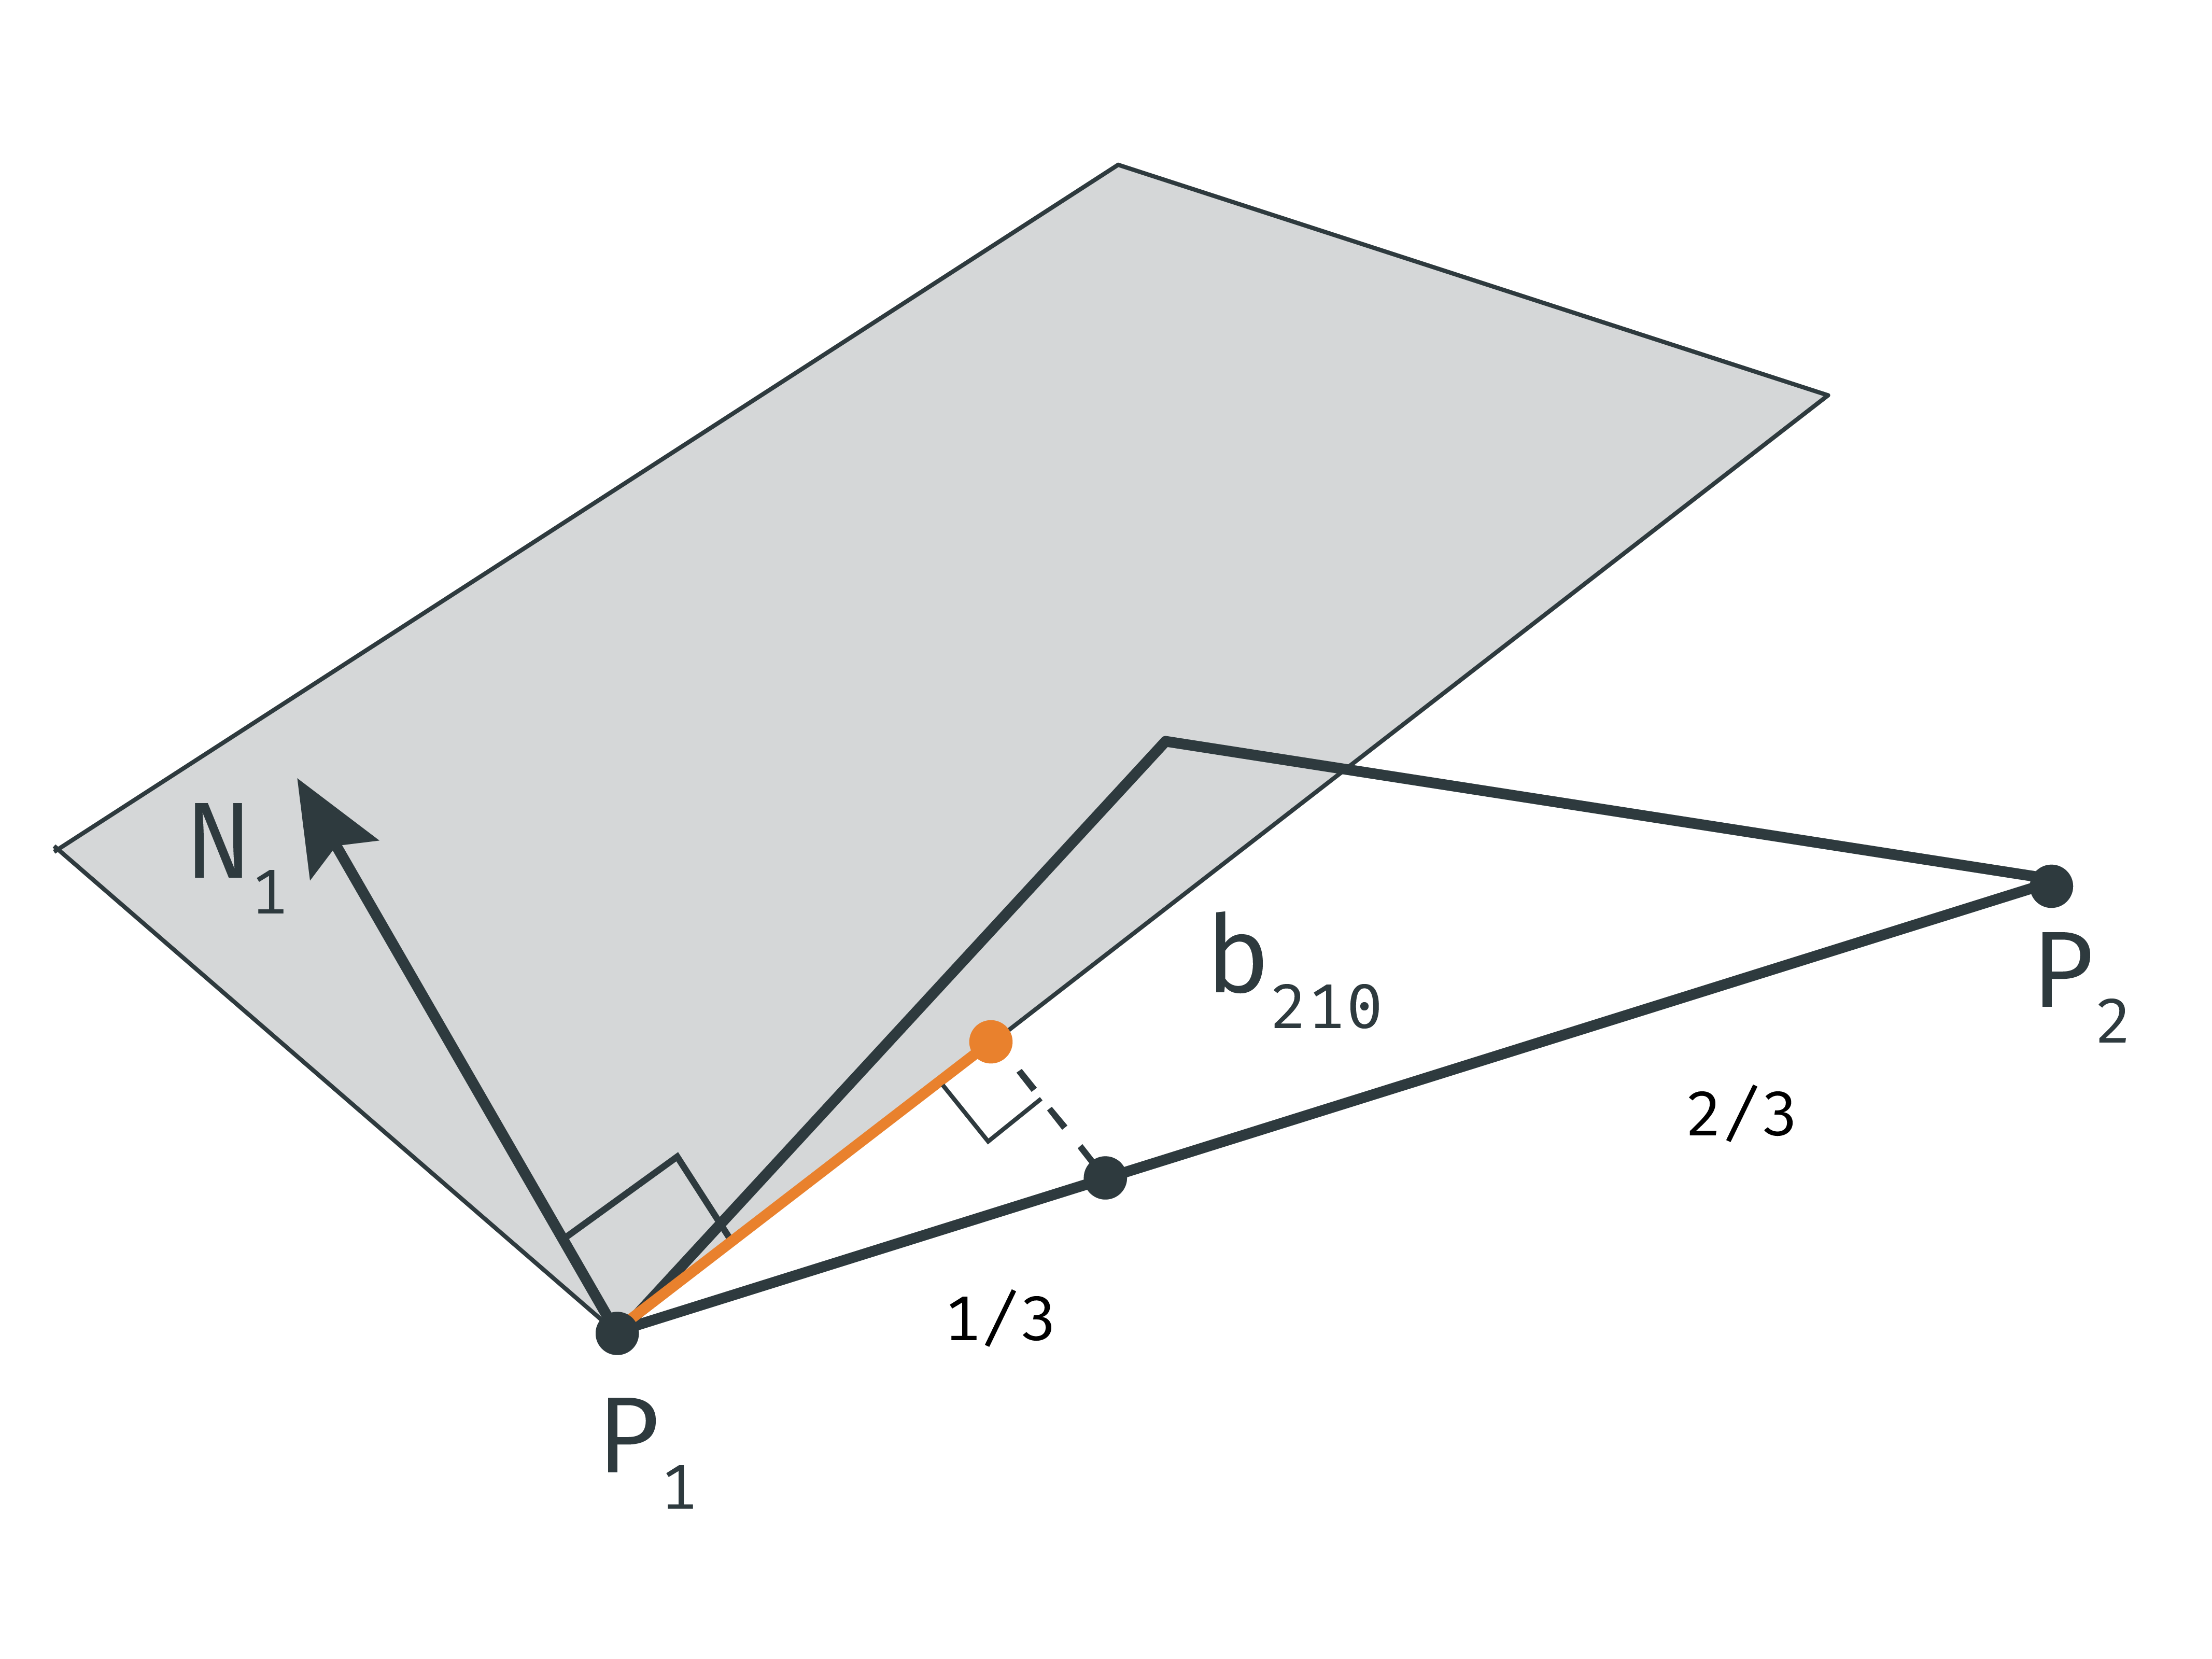
\includegraphics[width=\textwidth]{img/1_single/geometry_2.png}
				\small{normal projection}
				\end{center}
			\end{column}
			\uncover<2>{
				\begin{column}{0.4\textwidth}
					\begin{equation*}
						\begin{aligned}
						w_{ij} & = (P_j - P_i) \cdot N_i \in \mathbb{R} \\
						b_{210} & = \frac{2 P_1 + P_2 - w_{12}N1}{3},\\
						~ & \vdots \\
						b_{201} & = \frac{2 P_1 + P_3 - w_{13}N1}{3}
						\end{aligned}
					\end{equation*}
				\end{column}
			}
		\end{columns}
	\end{frame}

	% b_{120} & = (2 P_2 + P_1 - w_{21}N2) / 3,\\
	% b_{021} & = (2 P_2 + P_3 - w_{23}N2) / 3,\\
	% b_{012} & = (2 P_3 + P_2 - w_{32}N3) / 3,\\
	% b_{102} & = (2 P_3 + P_1 - w_{31}N3) / 3,\\

	\begin{frame}\frametitle{Geometry - Center Coefficient}
		\begin{columns}
			\begin{column}{0.6\textwidth}
				\begin{center}
				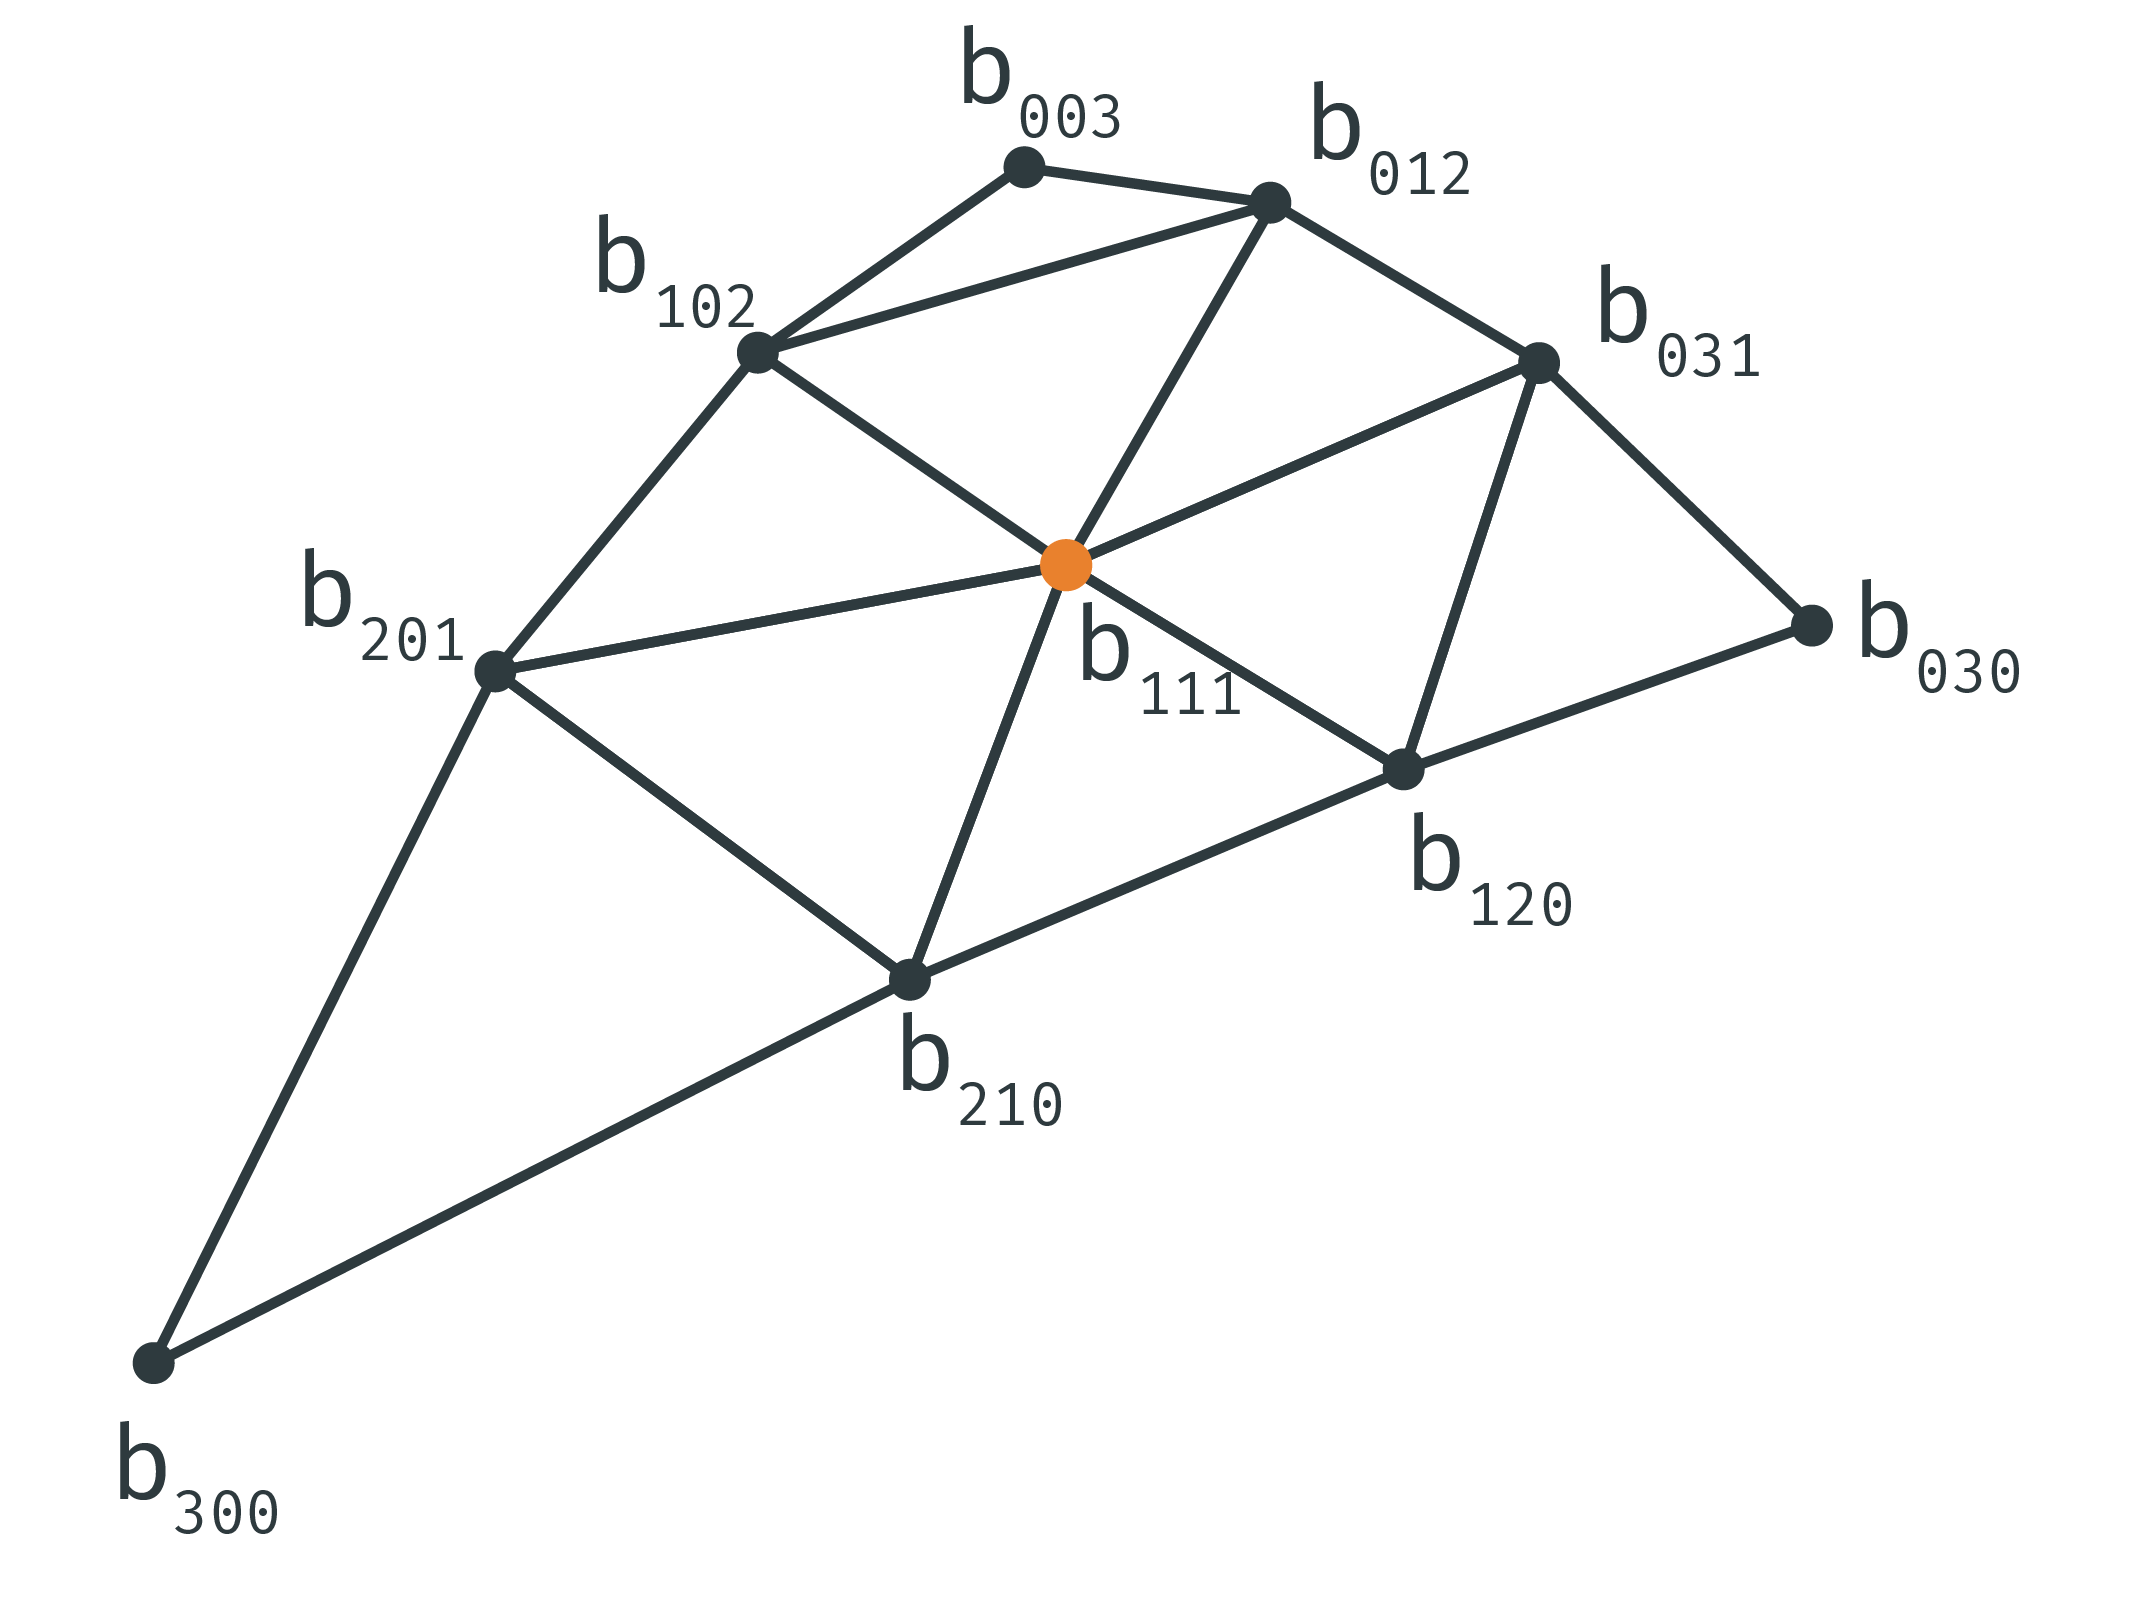
\includegraphics[width=\textwidth]{img/1_single/geometry_3.png}
				\small{center control point}
				\end{center}
			\end{column}
			\uncover<2>{
				\begin{column}{0.4\textwidth}	
					\begin{multline*}
					E = (b_{210} + b_{120} + b_{021} \\ 
					+ b_{012} + b_{102} + b_{201}) / 6,
					\end{multline*}
					\begin{equation*}
					\begin{aligned}
					V & = (P_1 + P_2 + P_3)/ 3, \\
					b_{111} & = E + (E - V) / 2
					\end{aligned}
					\end{equation*}
				\end{column}
			}
		\end{columns}
	\end{frame}	

	\begin{frame}\frametitle{Geometry - Result}
		\enhancement{Set result slide to plain}
		\begin{columns}
			\begin{column}{0.6\textwidth}
				\begin{center}
				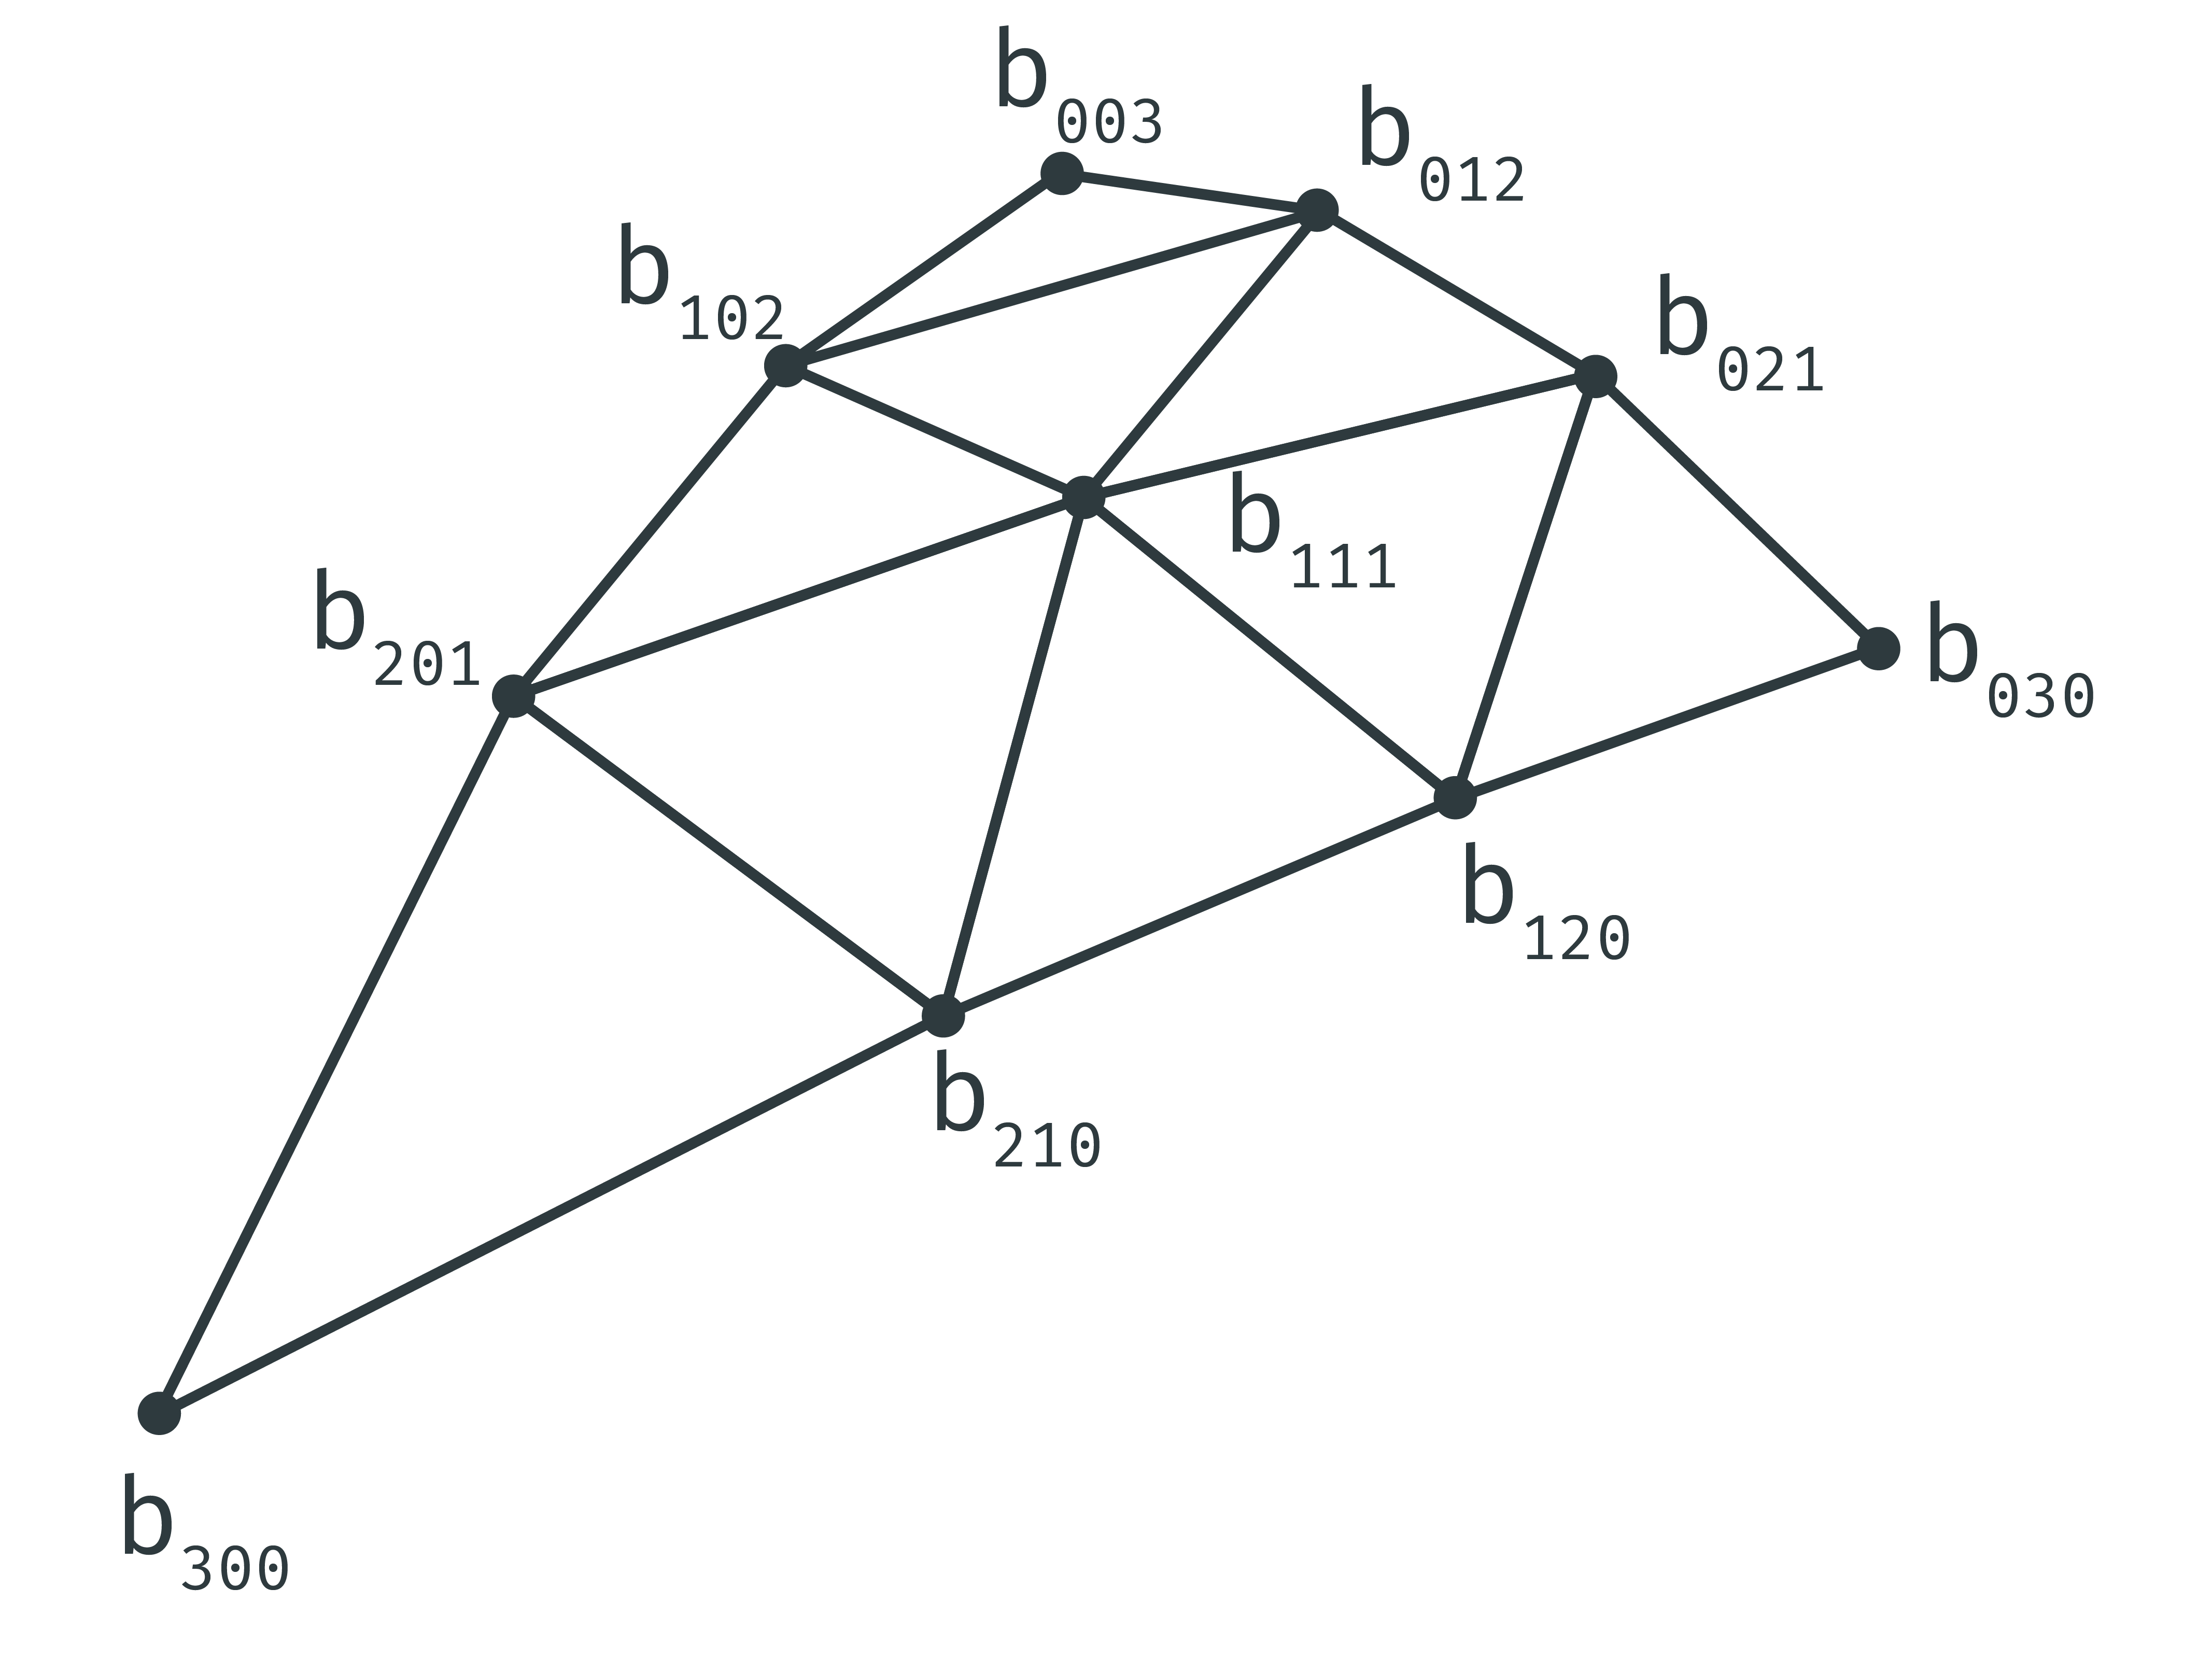
\includegraphics[width=\textwidth]{img/1_single/geometry_4.png}
				\end{center}	
			\end{column}
		\end{columns}
	\end{frame}

	\begin{frame}\frametitle{Overview}
		\begin{columns}
			\begin{column}{0.9\textwidth}
				\begin{center}
					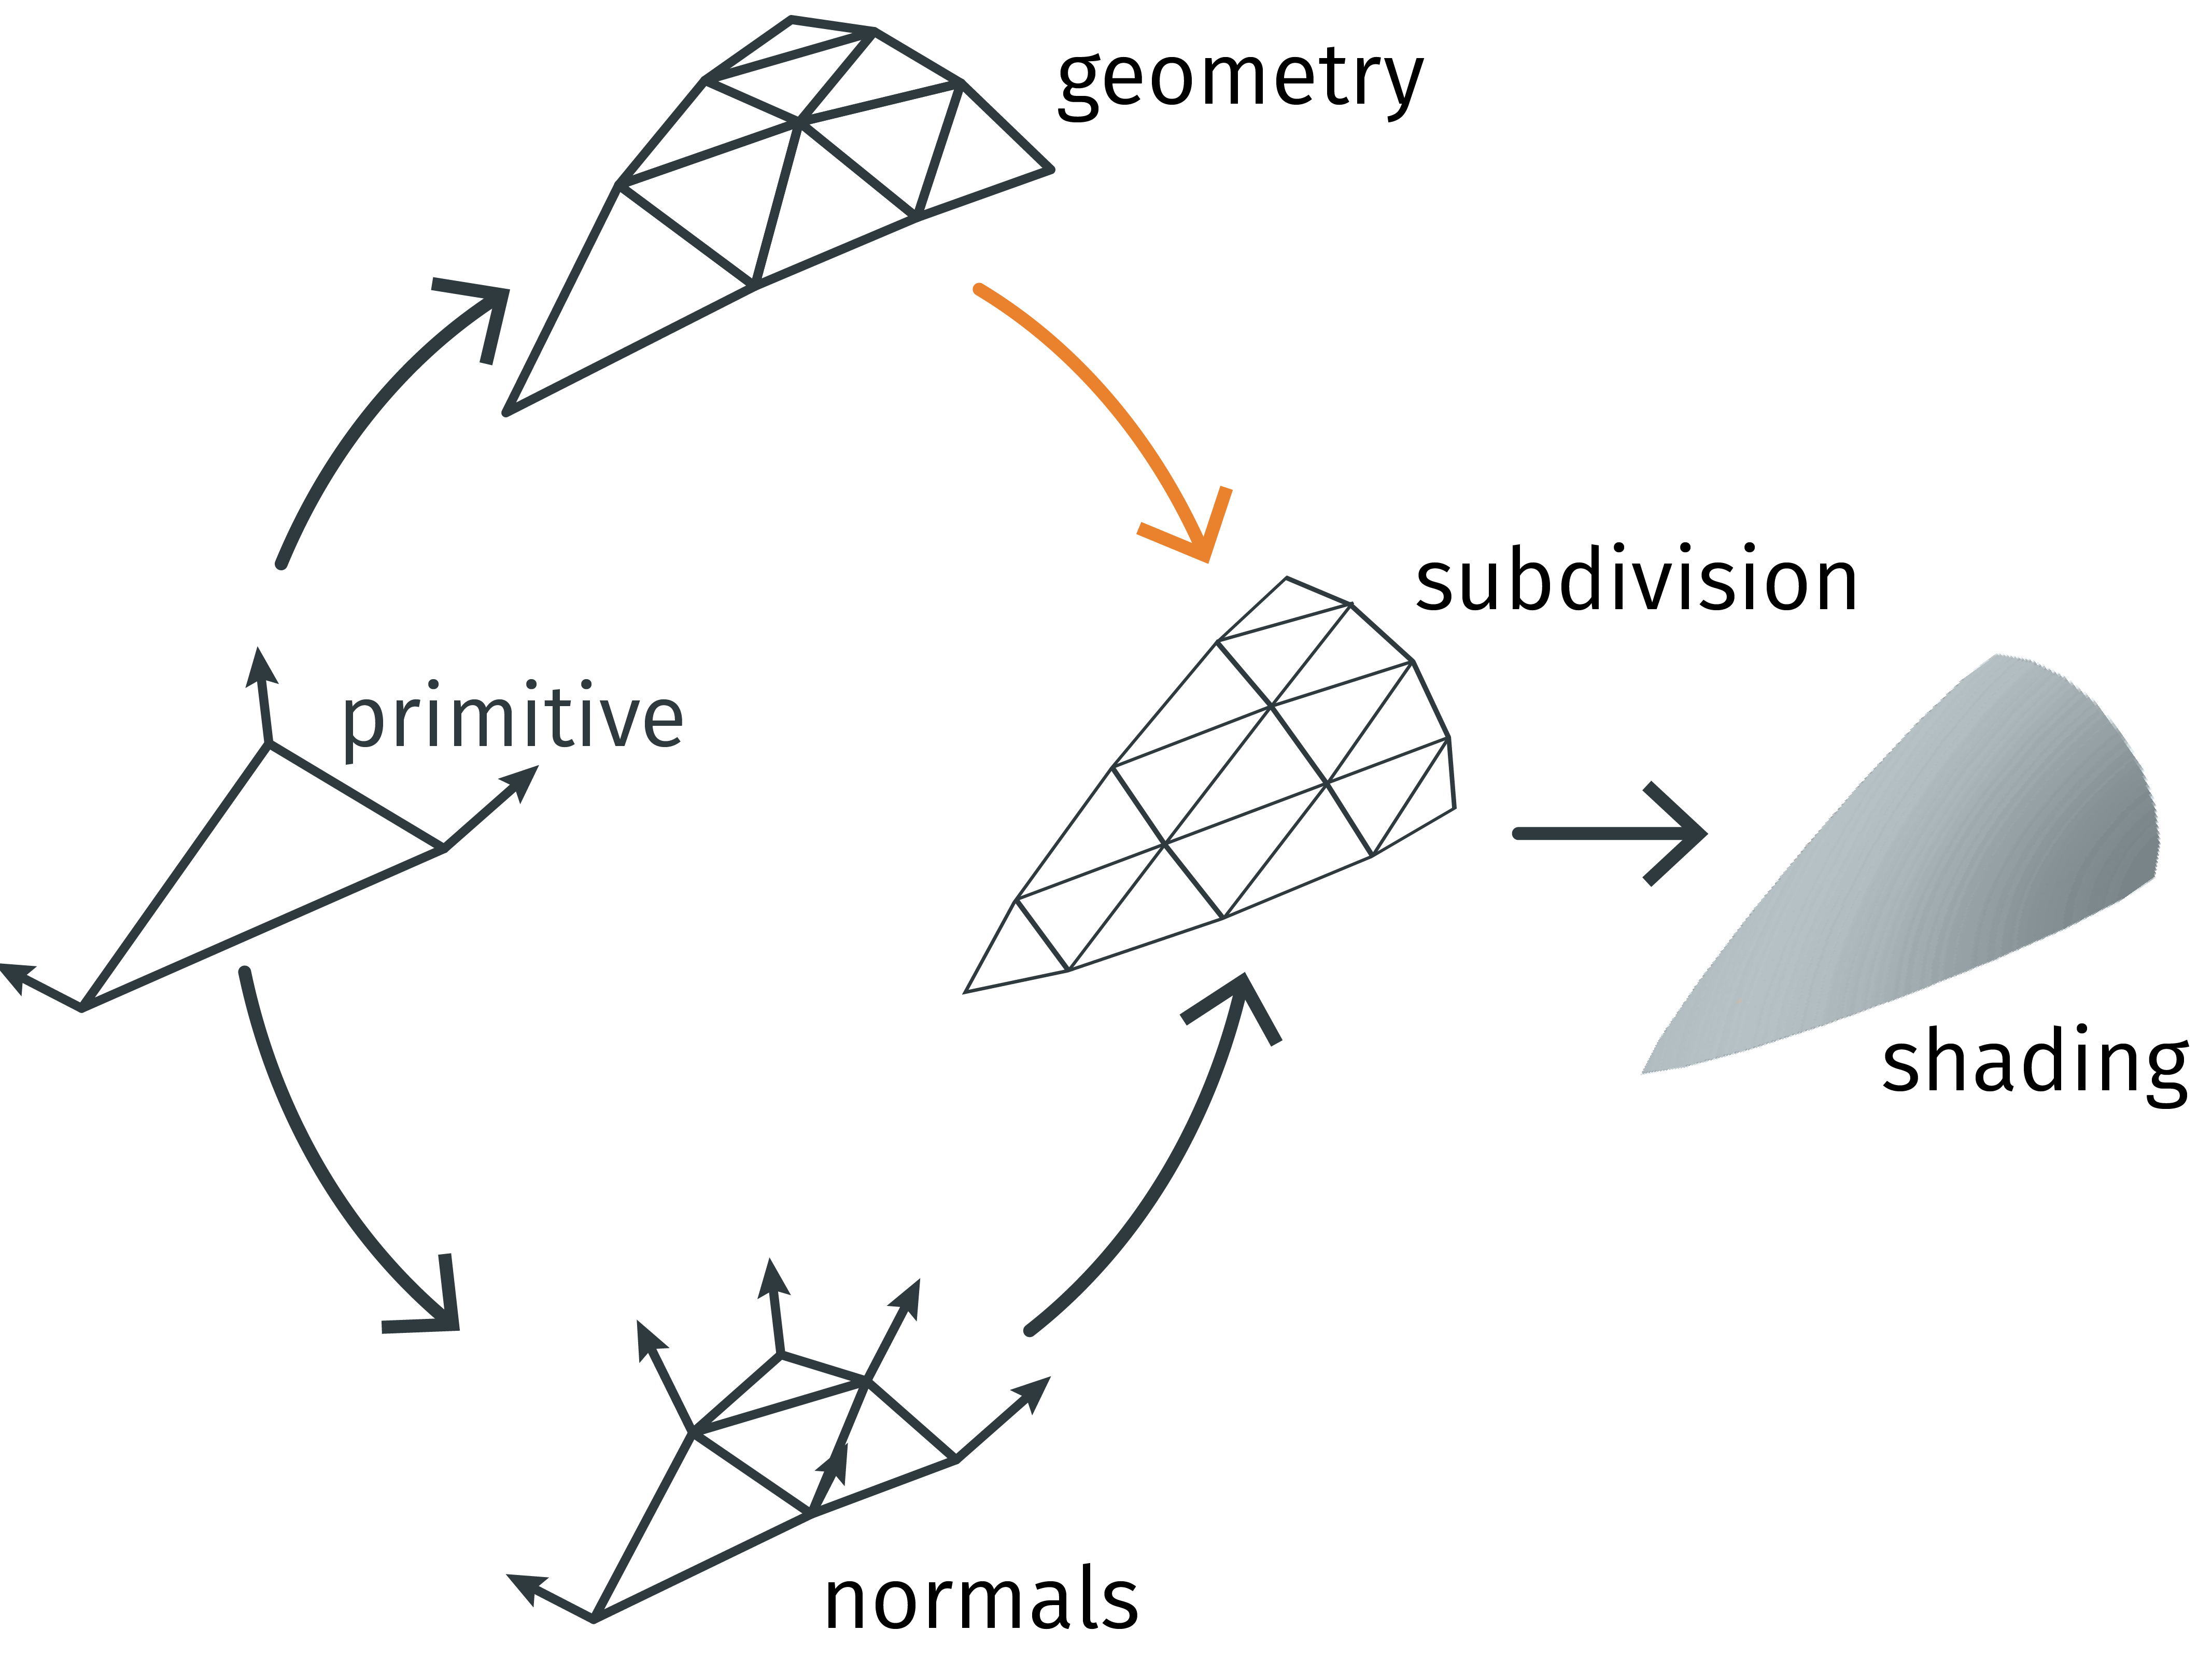
\includegraphics[width=\textwidth]{./img/1_single/recap_geomToShading.png}
				\end{center}		
			\end{column}
		\end{columns}
	\end{frame}	

	\begin{frame}\frametitle{Cubic patch}
	\todo[inline]{Spacing van de for all}
	\todo[inline]{Plaatje?}
		\begin{columns}
			\begin{column}{\textwidth}
				\begin{equation*}
					b: \mathbb{R}^2 \rightarrow \mathbb{R}^3 \text{, for } w = 1 - u - v, u, v \text{, } w \geq 0
				\end{equation*}
				\begin{equation*}
					\begin{aligned}
						b(u,v) & = \sum\limits_{i+j+k=3} b_{ijk} \frac{3!}{i!j!k!} u^i v^j w^k\\
						& = b_{300} w^3 + b_{030} u^3 + b_{003} v^3 \\
						& + b_{210} 3 w^2 u + b_{120} 3 w u^2 + b_{201} 3 w^2 v\\
						& + b_{021} 3 u^2 v + b_{102} 3 w v^2 + b_{012} 3 u v^2\\
						& + b_{111} 6 w u v.
 					\end{aligned}
				\end{equation*}
			\end{column}
		\end{columns}
	\end{frame}

		\begin{frame}\frametitle{Overview}
		% \todo[inline]{The steps. Recap of everything construct geometry and normals and evaluate less (low lod) or more points (high lod)}
		\begin{columns}
			\begin{column}{0.9\textwidth}
				\begin{center}	
					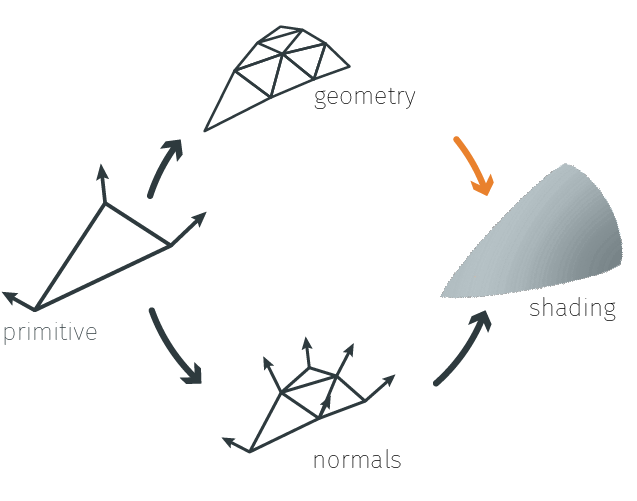
\includegraphics[width=\textwidth]{./img/1_single/recap_inputToNormals.png}
				\end{center}		
			\end{column}
		\end{columns}
	\end{frame}	

	\begin{frame}\frametitle{Normals}
	\enhancement{emphasize normals more}
		\begin{columns}
			\begin{column}{0.6\textwidth}
				\begin{center}
					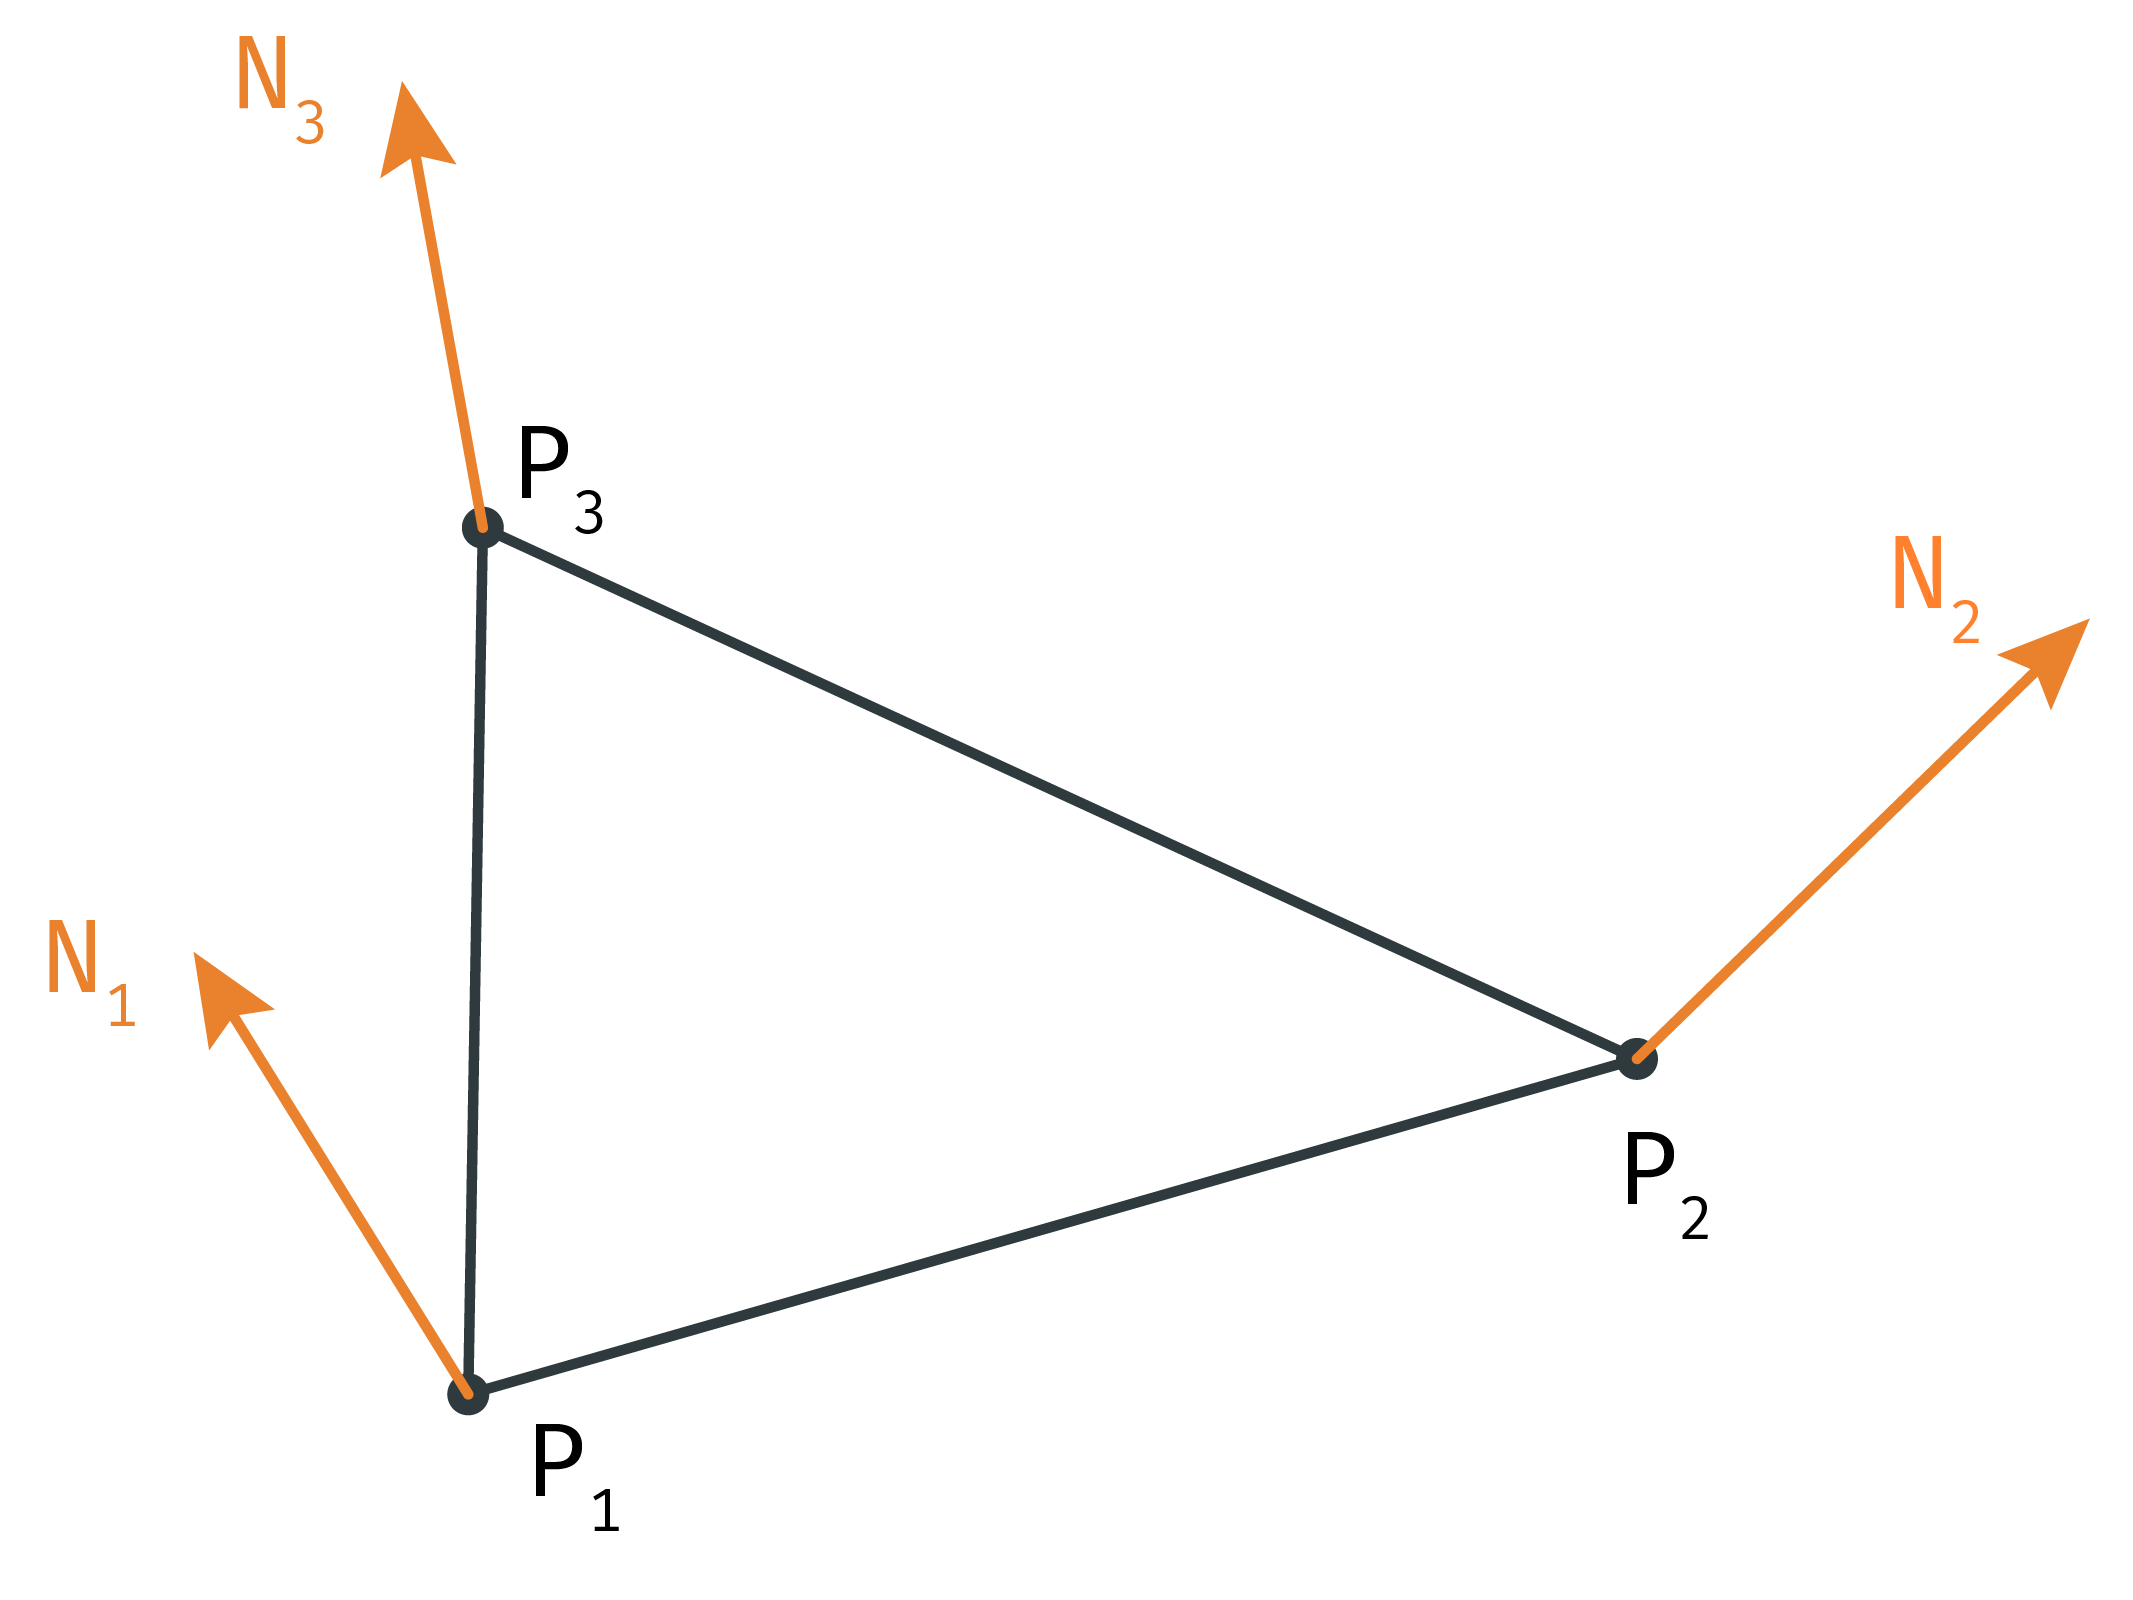
\includegraphics[width=\textwidth]{img/1_single/inputPrimitive_emphNormal.png}
					\small{input primitive}
				\end{center}
			\end{column}
		\end{columns}
	\end{frame}


	\begin{frame}\frametitle{Normals - theory}
		\begin{columns}
			\begin{column}{0.6\textwidth}
				\begin{center}
					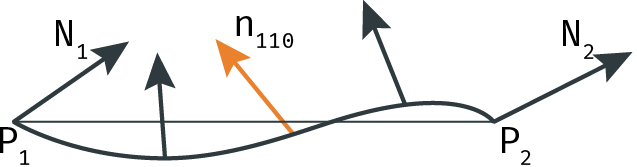
\includegraphics[width=\textwidth]{img/1_single/linearVsQuadraticNormals_linear.png}
					\small{linear}
				\end{center}	
			\end{column}
		\end{columns}
		\pause
		\vspace{0.8cm}
		\begin{columns}
			\begin{column}{0.6\textwidth}
				\begin{center}
					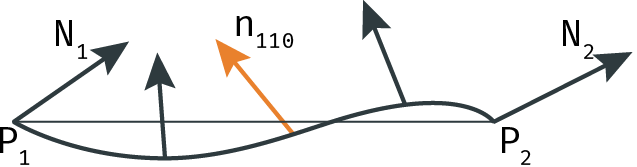
\includegraphics[width=\textwidth]{img/1_single/linearVsQuadraticNormals_quadratic.png}
					\small{quadratic}
				\end{center}	
			\end{column}
		\end{columns}
	\end{frame}

	\begin{frame}\frametitle{Normals - example}
		\begin{columns}
			\begin{column}{0.4\textwidth}
			\begin{center}
					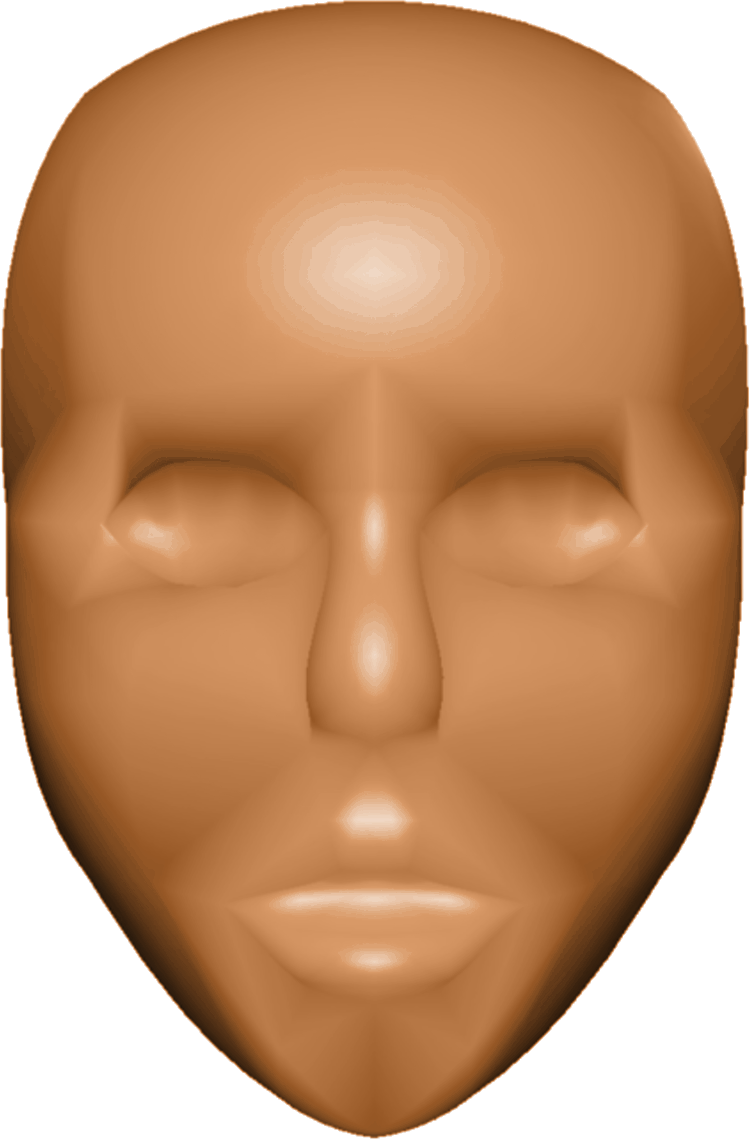
\includegraphics[width=\textwidth]{img/1_single/linearlyVaryingNormals.png}
					\small{linear}
				\end{center}	
			\end{column}
			\begin{column}{0.4\textwidth}
			\begin{center}
					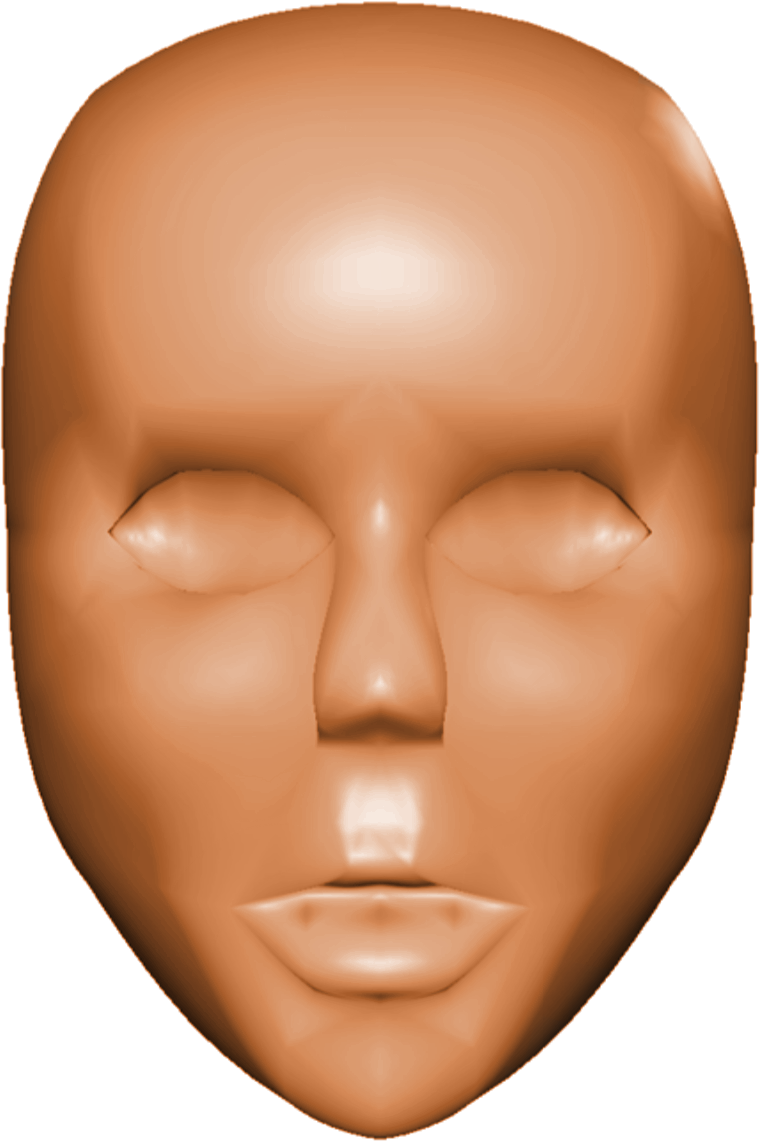
\includegraphics[width=\textwidth]{img/1_single/quadriticallyVaryingNormals.png}
					\small{quadratic}
				\end{center}	
			\end{column}
		\end{columns}
	\end{frame}


	\begin{frame}\frametitle{Normals - theory}
		\begin{columns}
			\begin{column}{0.6\textwidth}
				\begin{center}
					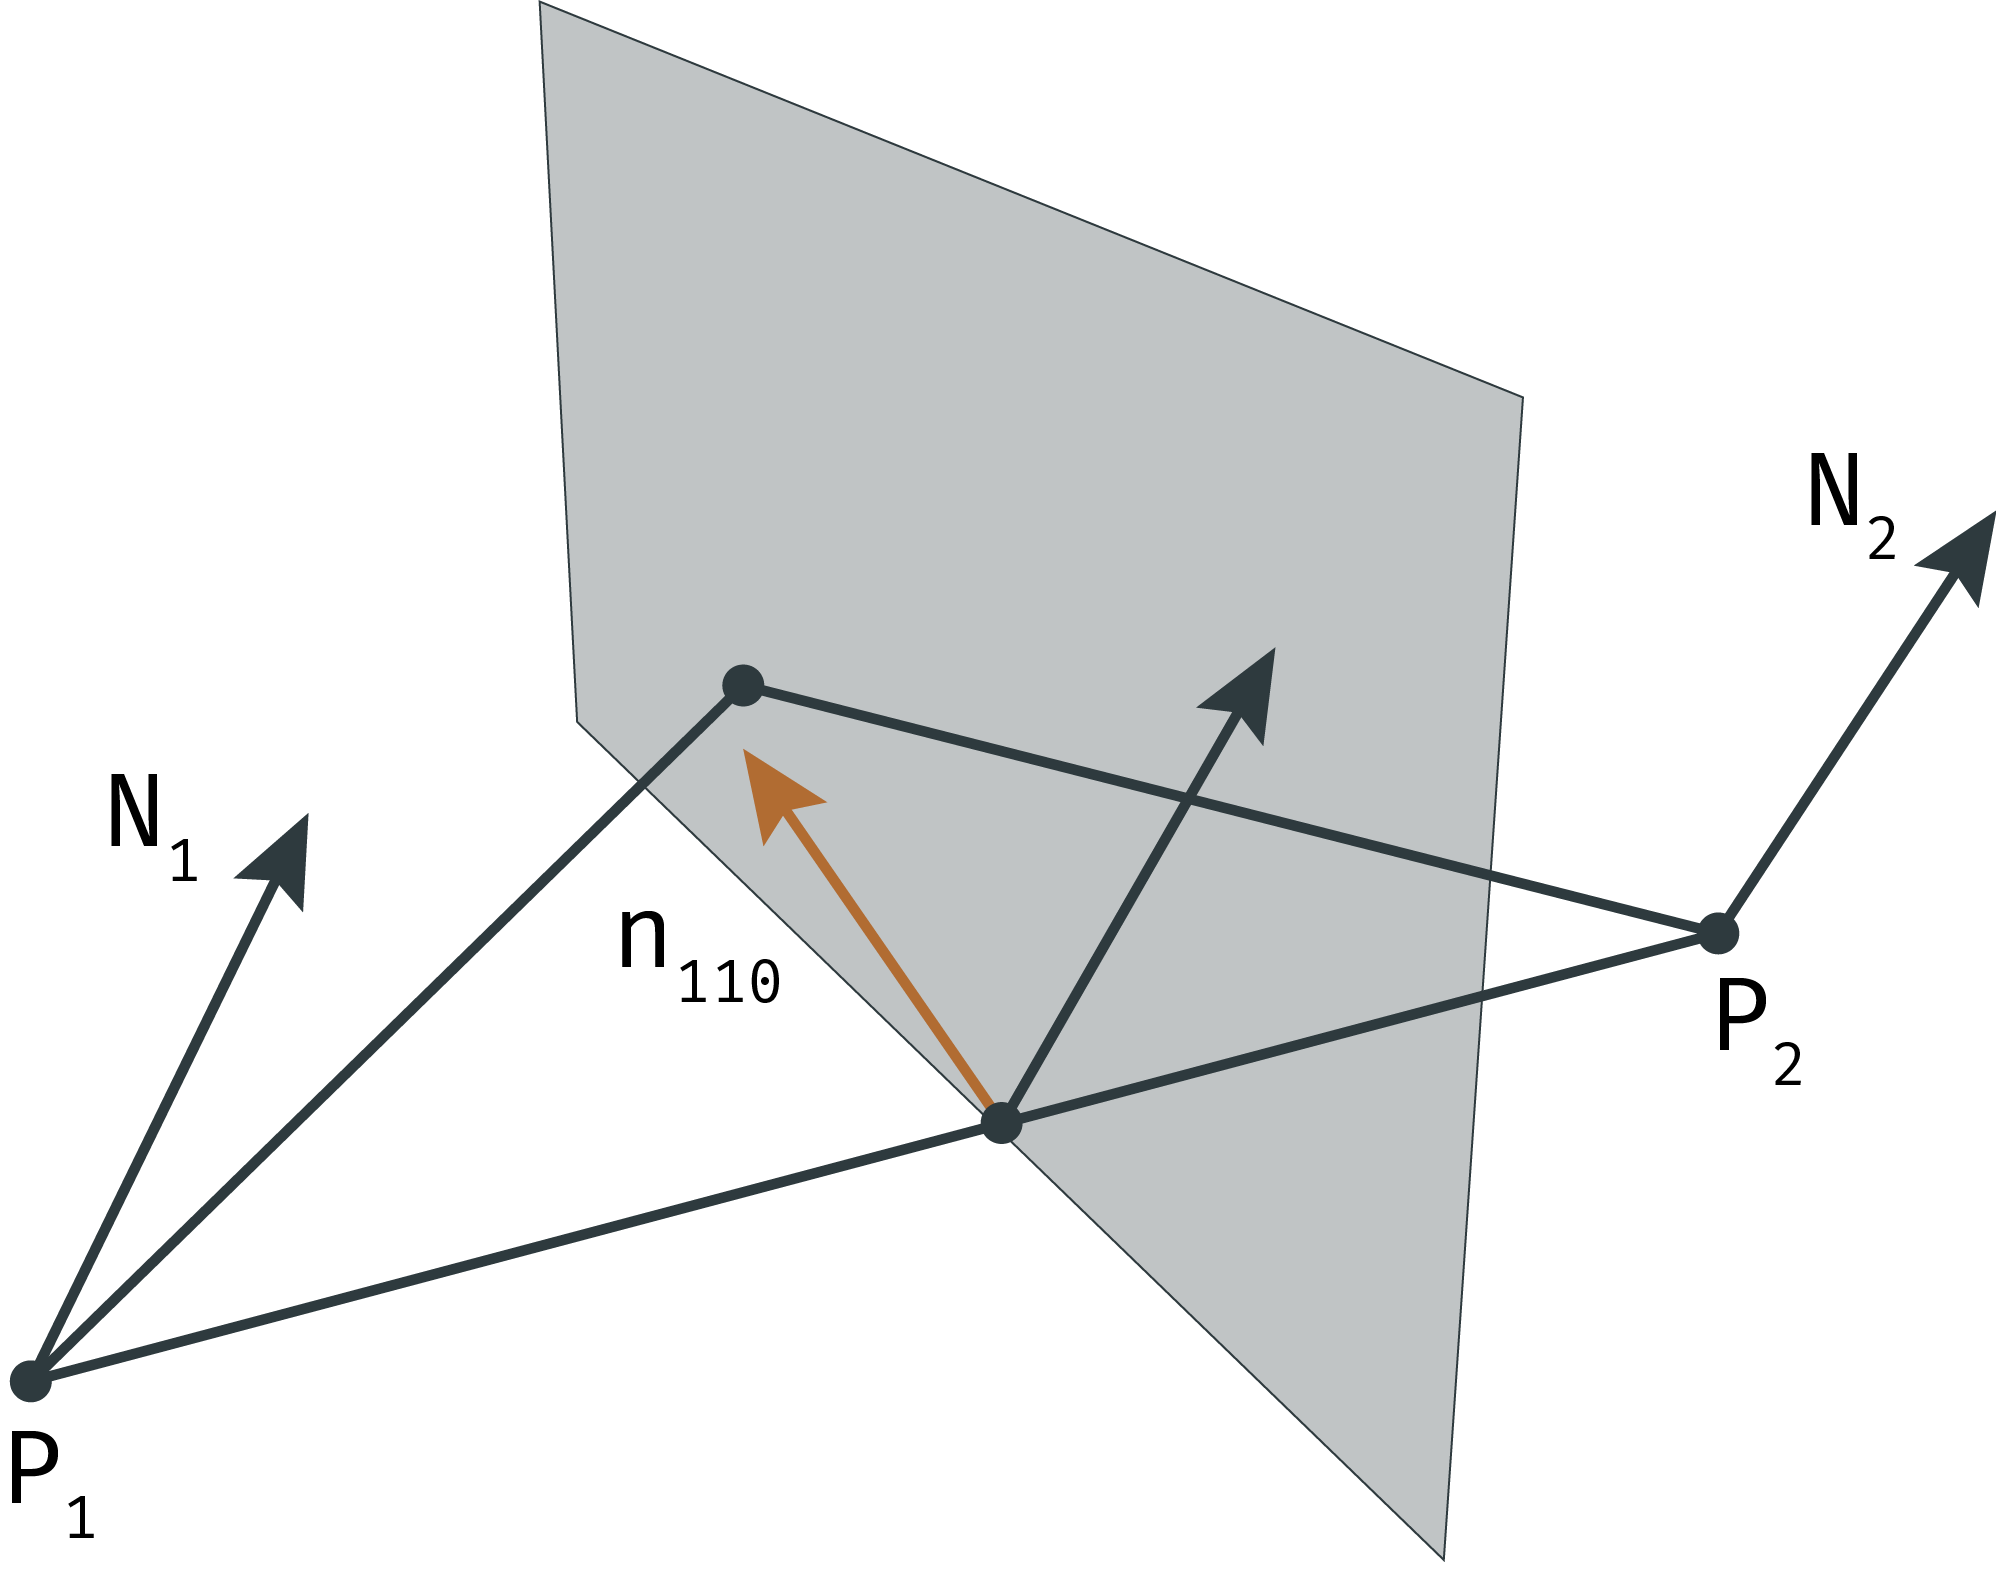
\includegraphics[width=\textwidth]{img/1_single/computingNormals.png}
				\end{center}
			\end{column}
		\end{columns}
		
		\begin{columns}
			\begin{column}{0.4\textwidth}
				\uncover<2>{
					\begin{equation*}
					\begin{aligned}
						v_{ij}  & = 2\frac{(P_j - P_i) \cdot (N_i + N_j)}{(P_j - P_i) \cdot (P_j - P_i)} \in \mathbb{R} \\
						h_{110} & = N_1 + N2 - v_{12}(P_2 - P_1)\\
						n_{110} & =	h_{110} / ||h_{110}||
					\end{aligned}
					\end{equation*}
				}
			\end{column}
		\end{columns}
	\end{frame}

	\begin{frame}
		\frametitle{Normals - result}
		\enhancement{Set result slide to plain}
		\begin{columns}
			\begin{column}{0.6\textwidth}
				\begin{center}
					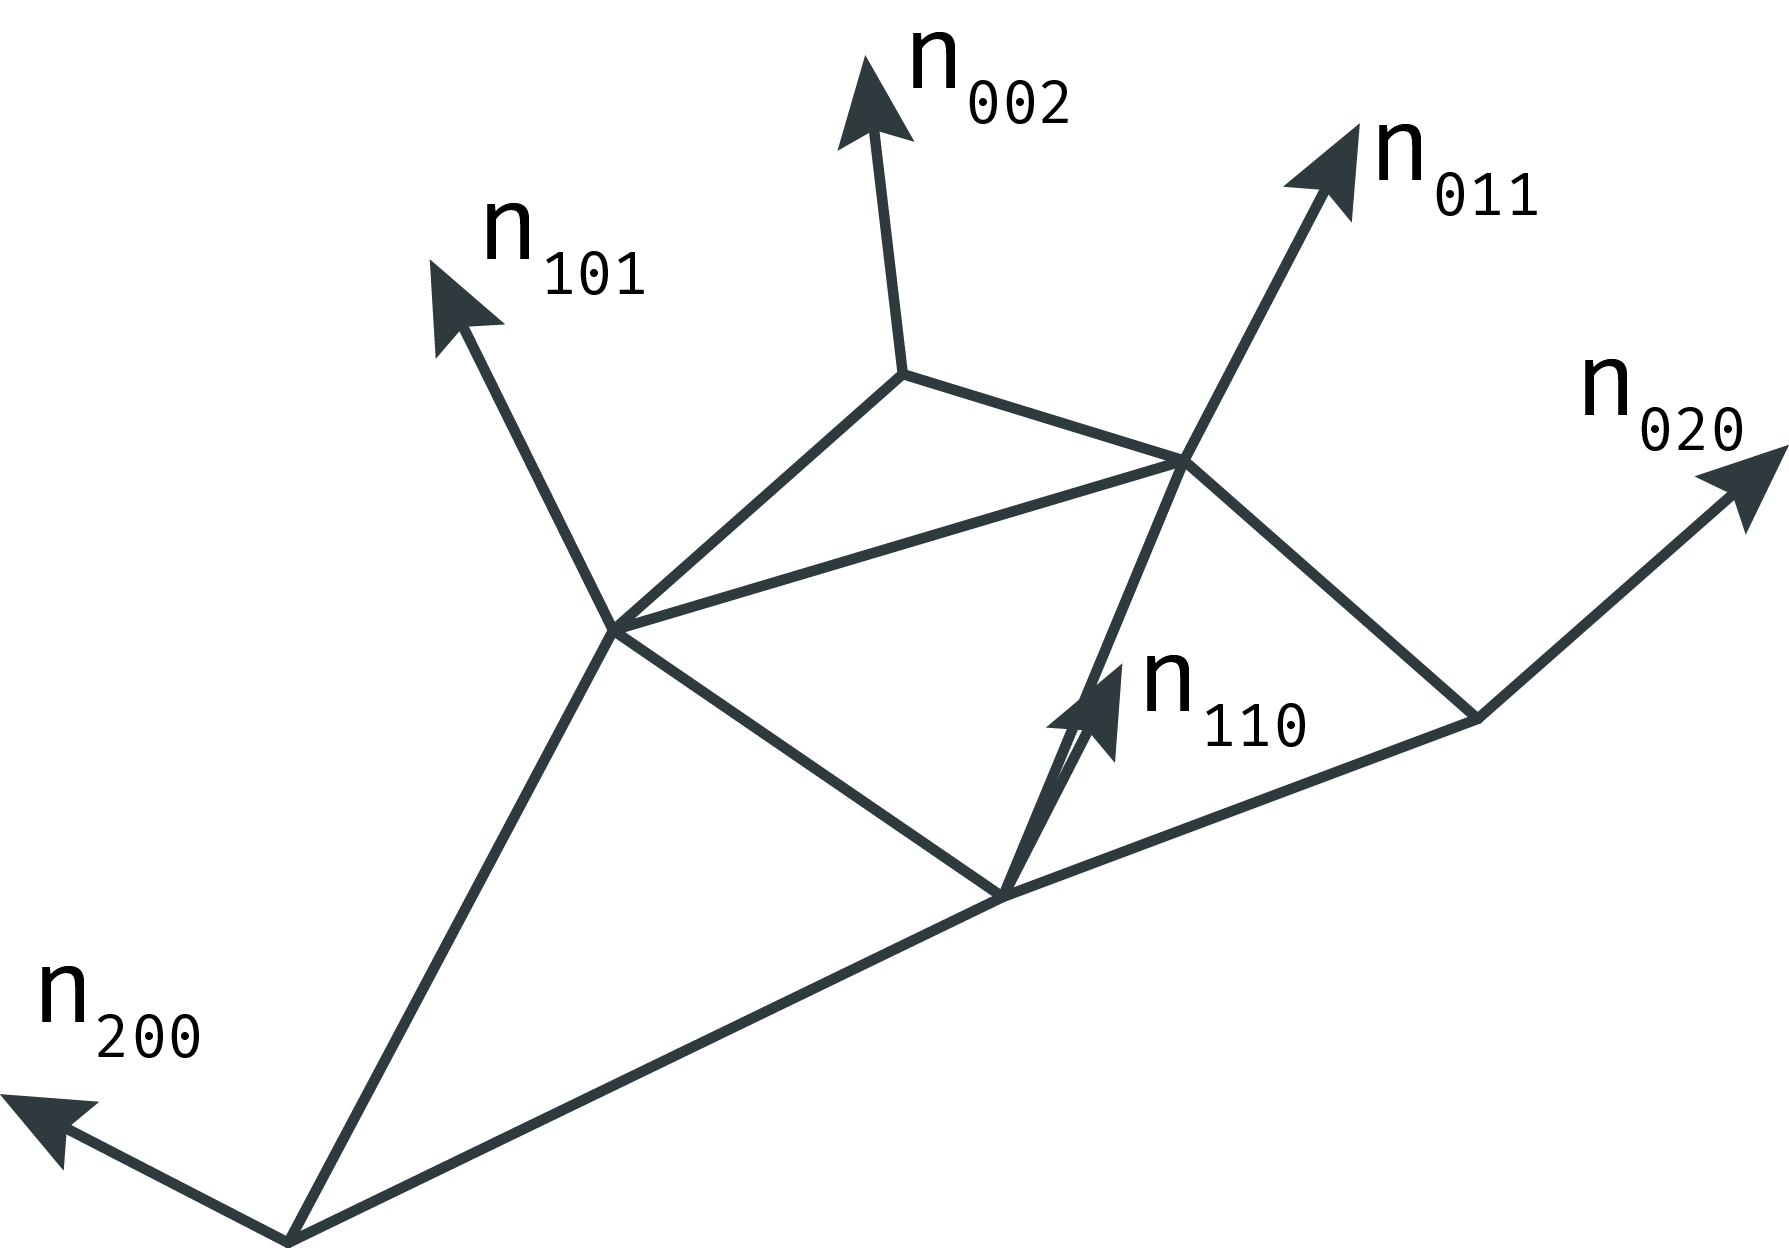
\includegraphics[width=\textwidth]{img/1_single/normals.png}
				\end{center}	
			\end{column}
		\end{columns}
	\end{frame}


	\begin{frame}\frametitle{Overview}
		% \todo[inline]{The steps. Recap of everything construct geometry and normals and evaluate less (low lod) or more points (high lod)}
		\begin{columns}
			\begin{column}{0.9\textwidth}
				\begin{center}
					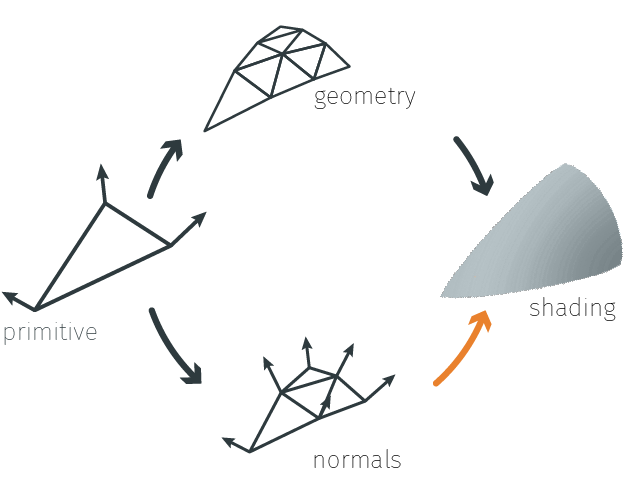
\includegraphics[width=\textwidth]{./img/1_single/recap_normalsToShading.png}
				\end{center}		
			\end{column}
		\end{columns}
	\end{frame}	


	\begin{frame}\frametitle{Quadratic Patch}
	\todo[inline]{Plaatje}
		\begin{equation*}
			n: \mathbb{R}^2 \rightarrow \mathbb{R}^3 \text{, for}\ w = 1 - u - v \text{,}\ u, v, w \geq 0 
		\end{equation*}
		\begin{equation*}
			\begin{aligned}
			n(u,v) & = \sum\limits_{i+j+k=2} n_{ijk} u^i v^j w^k\\
			& = n_{200} w^2 + n_{020} u^2 + n_{002} v^2\\
			& + n_{110} w u + n_{011} u v + n_{101} w v
			\end{aligned}
		\end{equation*}
	\end{frame}	

	\begin{frame}
		\frametitle{Level Of Detail}
		\begin{columns}
			\begin{column}[b]{0.22\textwidth}
				\begin{center}
					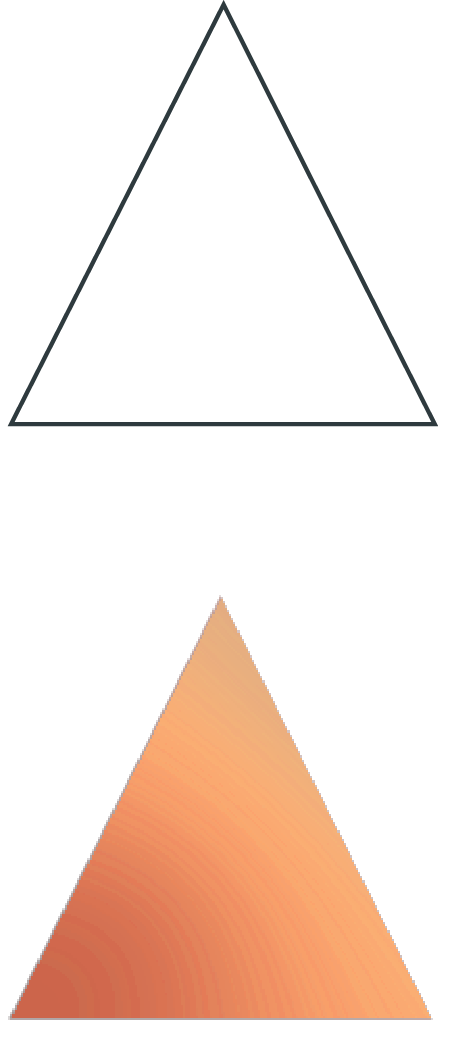
\includegraphics[width=\textwidth]{./img/1_single/lod_lod0.png}
					\small{0}
				\end{center}	
			\end{column}
			\begin{column}[b]{0.22\textwidth}
				\begin{center}
					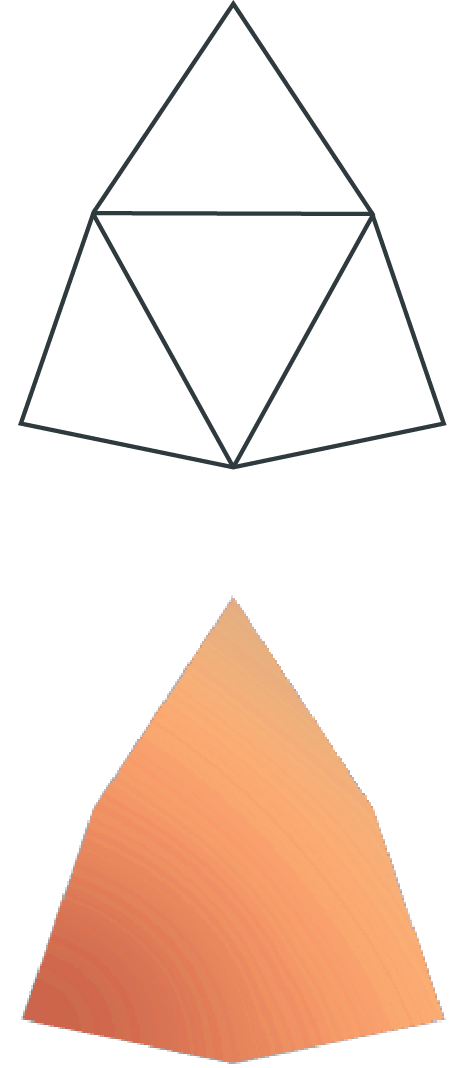
\includegraphics[width=\textwidth]{./img/1_single/lod_lod1.png}	
					\small{1}
				\end{center}	
			\end{column}
			\begin{column}[b]{0.22\textwidth}
				\begin{center}
					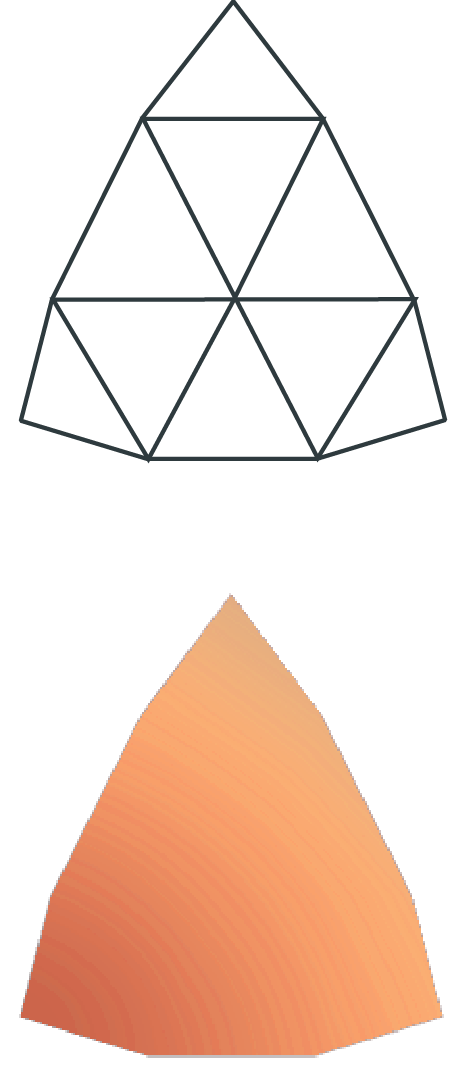
\includegraphics[width=\textwidth]{./img/1_single/lod_lod2.png}	
					\small{2}
				\end{center}	
			\end{column}
			\begin{column}[b]{0.22\textwidth}
				\begin{center}
					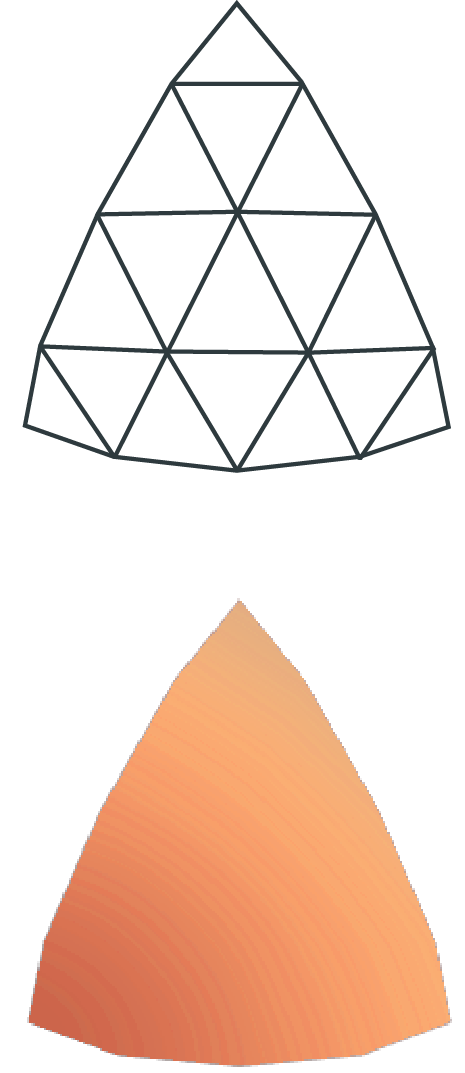
\includegraphics[width=\textwidth]{./img/1_single/lod_lod3.png}	
					\small{3}
				\end{center}	
			\end{column}
		\end{columns}
	\end{frame}	


	\begin{frame}\frametitle{Overview}
		% \todo[inline]{The steps. Recap of everything construct geometry and normals and evaluate less (low lod) or more points (high lod)}
		\begin{columns}
			\begin{column}{0.9\textwidth}
				\begin{center}
					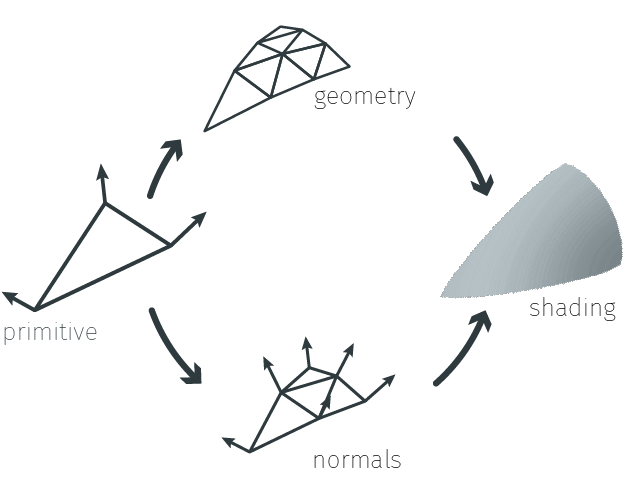
\includegraphics[width=\textwidth]{./img/1_single/recap_overview.png}
				\end{center}		
			\end{column}
		\end{columns}
	\end{frame}	
